\documentclass[journal]{IEEEtran}

\usepackage{cite}
%\usepackage[pdftex]{graphicx}
%\usepackage{graphics} % for pdf, bitmapped graphics files
\usepackage{epsfig} % for postscript graphics files
\usepackage{mathptmx} % assumes new font selection scheme installed
\usepackage{times} % assumes new font selection scheme installed
\usepackage[cmex10]{amsmath} % assumes amsmath package installed
%\usepackage{gensymb} %helps for math symbols
\usepackage{textcomp} %helps with math symbols

%\usepackage{subfig}
\usepackage{graphicx}
\usepackage{caption}
\usepackage{subcaption}


\usepackage{amssymb}  % assumes amsmath package installed
\usepackage{multirow}
\usepackage{array}
\usepackage{mdwtab}
\usepackage{bigstrut}
	


% correct bad hyphenation here
\hyphenation{op-tical net-works semi-conduc-tor}


\begin{document}
%
% paper title
% can use linebreaks \\ within to get better formatting as desired
\title{An Experimental Approach to AUV Dynamic Adaptive Sampling}


\author{Andres~Mora, Colin~Ho, and~Srikanth~Saripalli% <-this % stops a space
\thanks{A. Mora is with the School of Earth and Space Exploration, Arizona University,
550 E. Tyler Mall, Tempe, Arizona, 85287- USA e-mail: amoravar@asu.edu.}% <-this % stops a space
\thanks{*This work was supported in part by NSF grant XYZ}% <-this % stops a space
\thanks{Manuscript received April 21, 2012; revised January 11, 2007.}}

%\IEEEspecialpapernotice{(Invited paper)}

% The paper headers
\markboth{Journal of \LaTeX\ Class Files,~Vol.~xx, No.~xx, xx~2012}%
{Mora \MakeLowercase{\textit{et al.}}: Bare Demo of IEEEtran.cls for Journals}

	
% make the title area
\maketitle


\begin{abstract}
A critical problem in planning sampling paths for autonomous underwater vehicles is balancing obtaining an accurate scalar field estimation against efficiently utilizing the stored energy capacity of the sampling vehicle. 
Adaptive sampling approaches can only provide solutions when real-time and a priori environmental data is available. 
Through utilizing a cost-evaluation function to experimentally evaluate various sampling path strategies for a wide range of scalar fields and sampling densities, it is found that a systematic spiral sampling path strategy is optimal for high-variance scalar fields for all sampling densities and low-variance scalar fields when sampling is sparse. 
The random spiral sampling path strategy is found to be optimal for low-variance scalar fields when sampling is dense.
\end{abstract}

% Note that keywords are not normally used for peerreview papers.
\begin{IEEEkeywords}
Sampling, AUV, kriging
\end{IEEEkeywords}


% For peer review papers, you can put extra information on the cover
% page as needed:
% \ifCLASSOPTIONpeerreview
% \begin{center} \bfseries EDICS Category: 3-BBND \end{center}
% \fi
%
% For peerreview papers, this IEEEtran command inserts a page break and
% creates the second title. It will be ignored for other modes.
\IEEEpeerreviewmaketitle


%%%%%%%%%%%%%%%%%%%%%%%%%%%%%%%%%%%%%%%%%%%%%%%%%%%%%%%%%%%%%%%%%%%%%%%%%%%%%%%%
\section{Introduction}
\IEEEPARstart{A}{utonomous} underwater vehicles (AUV) are mobile robotic platforms that are utilized for environmental sampling, sensing and are capable of operating in a multitude of underwater aquatic environments \cite{forrest:investigation}.
In research they are commonly used to carry hydrological, geophysical, and/or biological sensor payloads that are used to gather remote and in-situ data to aid the study of open and closed aquatic bodies \cite{stoker:exploration}, \cite{german:hydro}.

An autonomous underwater vehicle is generally described as being capable of operation without any human controller; thus it must be able to traverse the aquatic environment on a desired path through autonomous navigation and control \cite{kumagai:newAUV}. 
The autonomous underwater vehicle used to collect the data analized in this paper is shown in Figure \ref{fig:iverAtPleasant}. 	

The goal of environmental sampling and sensing is to generate an accurate estimate of the underlying scalar field(s) over an area of interest. 
Generally, an estimate is generated by interpolating the sensing data collected over the area being studied. 
In the case of aquatic environments, a mobile vehicle can be introduced for it to autonomously collect the necessary sensing data. 

However a number of questions may be faced in order to gather these data.
When using an AUV as sensing platform its range is limited by the amount of stored energy it carries aboard. 
The problem of environmental sensing then becomes determining how one obtains an accurate estimation of the scalar field of interest while being constrained by the amount of stored energy the vehicle can utilize in order to sample the scalar field.
Moreover, what sampling pattern should be used to accurately determine the underlying scalar field?
How and under which conditions shall a particular sampling pattern be performed?
What are the parameters that constraint such selection?
Furthermore, is it possible to estimate the values of the underlying scalar field of an area in the future based on previous measurements taken from nearby locations?

\begin{figure}[htp]
	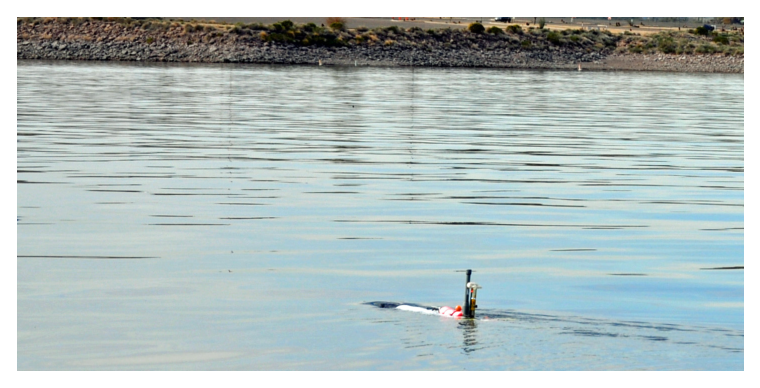
\includegraphics[width=\columnwidth, scale= 0.6]{figs/iverAtPleasant}
	\caption{Modified OceanServer IVER2 AUV at Lake Pleasant.}
	\label{fig:iverAtPleasant}
\end{figure} 

The purpose of this paper is to experimentally evaluate sampling strategies based upon estimation accuracy and energy consumption.
The paper also shows the result of a scalar field estimation of a given area based on the measurements previously gathered at a different nearby location.
 
The evaluation of the sampling strategies is conducted with a cost-evaluation function that considers multiple parameters (such as the AUV's power consumption), and can assign priorities to each factor. 
Incorporating a dynamical model of the AUV rather than a simplified energy consumption model to the proposed cost-evaluation function, allows to relax the assumptions made of its movement and provides a better approximation of the vehicle's power consumption performance during a given sampling path.
The evaluation takes into account real world and simulated isotropic, anisotropic scalar fields, as well as varying sampling densities to determine which sampling strategy is optimal for different scalar field types, for a range of sampling densities. 
The sampling path strategies evaluated in this study were systematic and stratified random sampling distributions with spiral and lawn mower sampling paths.

The research presented in this paper follows the flow presented in Figure \ref{fig:paperFlowExplanation}.
After having gathering in-situ data, we can observe the underlying scalar field present at data sampling area.
Based on the data sets obtained, we produce different sampling strategies over the underlying scalar field.
At this point we evaluate two important factors: the energy consumption of the vehicle and the error in the estimation of a scalar field obtained from the data set.
Finally, we can determine the which of the studied sampling patterns is the best one while considering a particular scalar field and the energy it consumes.   

Through utilizing the cost-evaluation function, it is found that the systematic spiral sampling path strategy best optimizes the energy consumption with the scalar reconstruction error compared to the other sampling path strategies evaluated. 
Additionally, it is found that the systematic spiral path consumes the least amount of energy out of the sampling path strategies evaluated.

\begin{figure}[htp]
	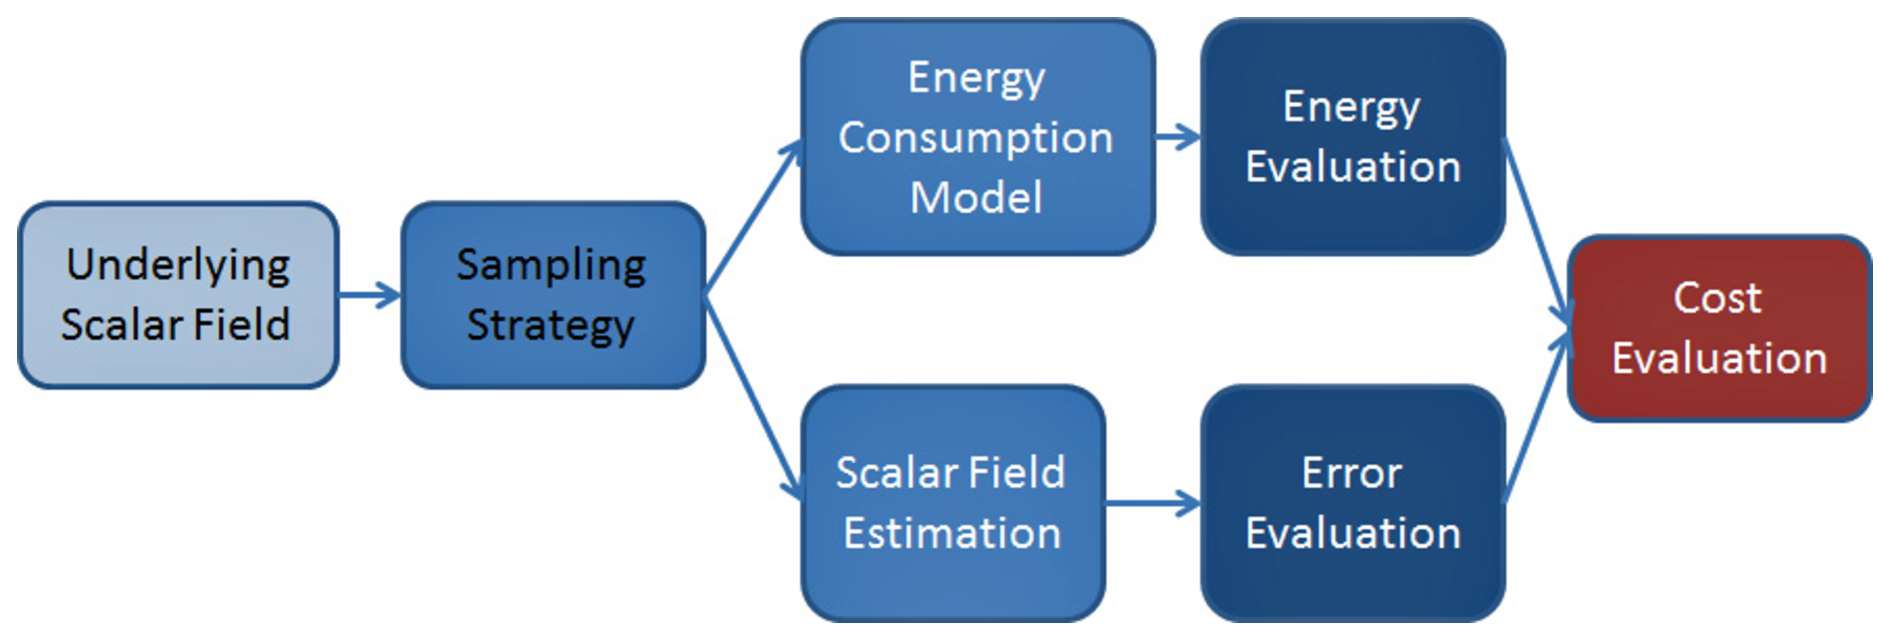
\includegraphics[width=\columnwidth, scale= 1.0]{figs/paperFlowExplanation}
	\caption{Experiment and analysis general description.}
	\label{fig:paperFlowExplanation}
\end{figure}

%%%%%%%%%%%%%%%%%%%%%%%%%%%%%%%%%%%%%%%%%%%5
\section{Related Work}
\label{relWork}

\subsection{Sampling Estimation}
In the fields of robotics, hydrology, geology, and geostatistical sciences, optimal sample collection and path planning are an active area of research \cite{mcbratney:exploration}. 
There is much prior and current work ongoing in the domain of path planning and sampling optimization for autonomous vehicles. 
For example, adaptive sampling algorithms have been developed that can direct the path of single or multiple autonomous underwater vehicles in towards locations of high probable data yield \cite{popa:adaptive}, and can be used in conjunction with existing sensor networks \cite{zhang:adaptive}. 
Additionally, energy optimal paths can be computed based upon known and sensed external variables such as ocean currents \cite{witt:go}-\cite{smith:autonomous}, and static or dynamic obstacles \cite{caldwell:reconfiguring}.


\subsection{Optimal Mobile Robotic Sampling}
However all of these planning schemes require a priori knowledge of the environment or real time sensing and data feedback. 
There are many AUV deployments scenarios where there is a lack of a priori data on the environment, and the AUV is equipped with sensors that do not provide real time data (such as taking physical water samples) \cite{stoker:exploration}. 
Therefore, in many real world deployments, the paths chosen are often simple lawnmower patterns that may or may not be optimal for the situation they are being utilized \cite{forrest:investigation}, \cite{stoker:exploration}. 
The evaluation conducted in this paper is targeted at looking at autonomous underwater vehicle path planning from an experimental field scientist�s data sampling perspective. 
The goal is to comparatively evaluate various sampling path strategies using a cost-evaluation function that can optimize multiple parameters. 
These results from this evaluation will aid choosing the best sampling path strategy for unknown scalar fields, with no real time data feedback.

\section{Scalar Fields and Kriging Approach}
\label{concepts}


\section{Experimental Setup}
\label{expSetup}

\subsection{AUV Platform: IVER}
Our AUV platform is based on the MIT-developed aquatic robotic platform called ``IVER2 Ocean Server''.
This robotic platform has a diameter of $14.7$[cm], a length of $127$[cm], it weights $20$[kg] approximately, and it has a maximum operation depth of $100$[m]. 

It has several navigational and environmental sensors onboard: GPS, CTD unit, sonar and our group has modified it such that its body can accomodate several cameras that are used during mapping tasks.
The platform is powered by a set of $95$[WHr], $14.4$[V], $6.6$[Ah] Li-Ion smart battery packs.
It has 4 independent fins making it possible to control the robot's yaw, pitch and allowing for an active roll correction. 
Its propulsion is based on a direct drive DC brushless motor. 

It also has two main computers on-board (based on an Intel ATOM 1.6[GHz]) that are in charge of navigation and mapping tasks.
The robot can be given commands remotely through its WiFi access point within a 1[km] range; in the event of an emergency the vehicle can be then commanded to stop its mission and go back to safety.

The robotic platform and its instrumentation payload used in this research are shown in Figure \ref{fig:iver}-\ref{fig:ysiSonde}. 

\begin{figure}
\centering
	\begin{subfigure}[t]{0.485\textwidth}
    	\centering
        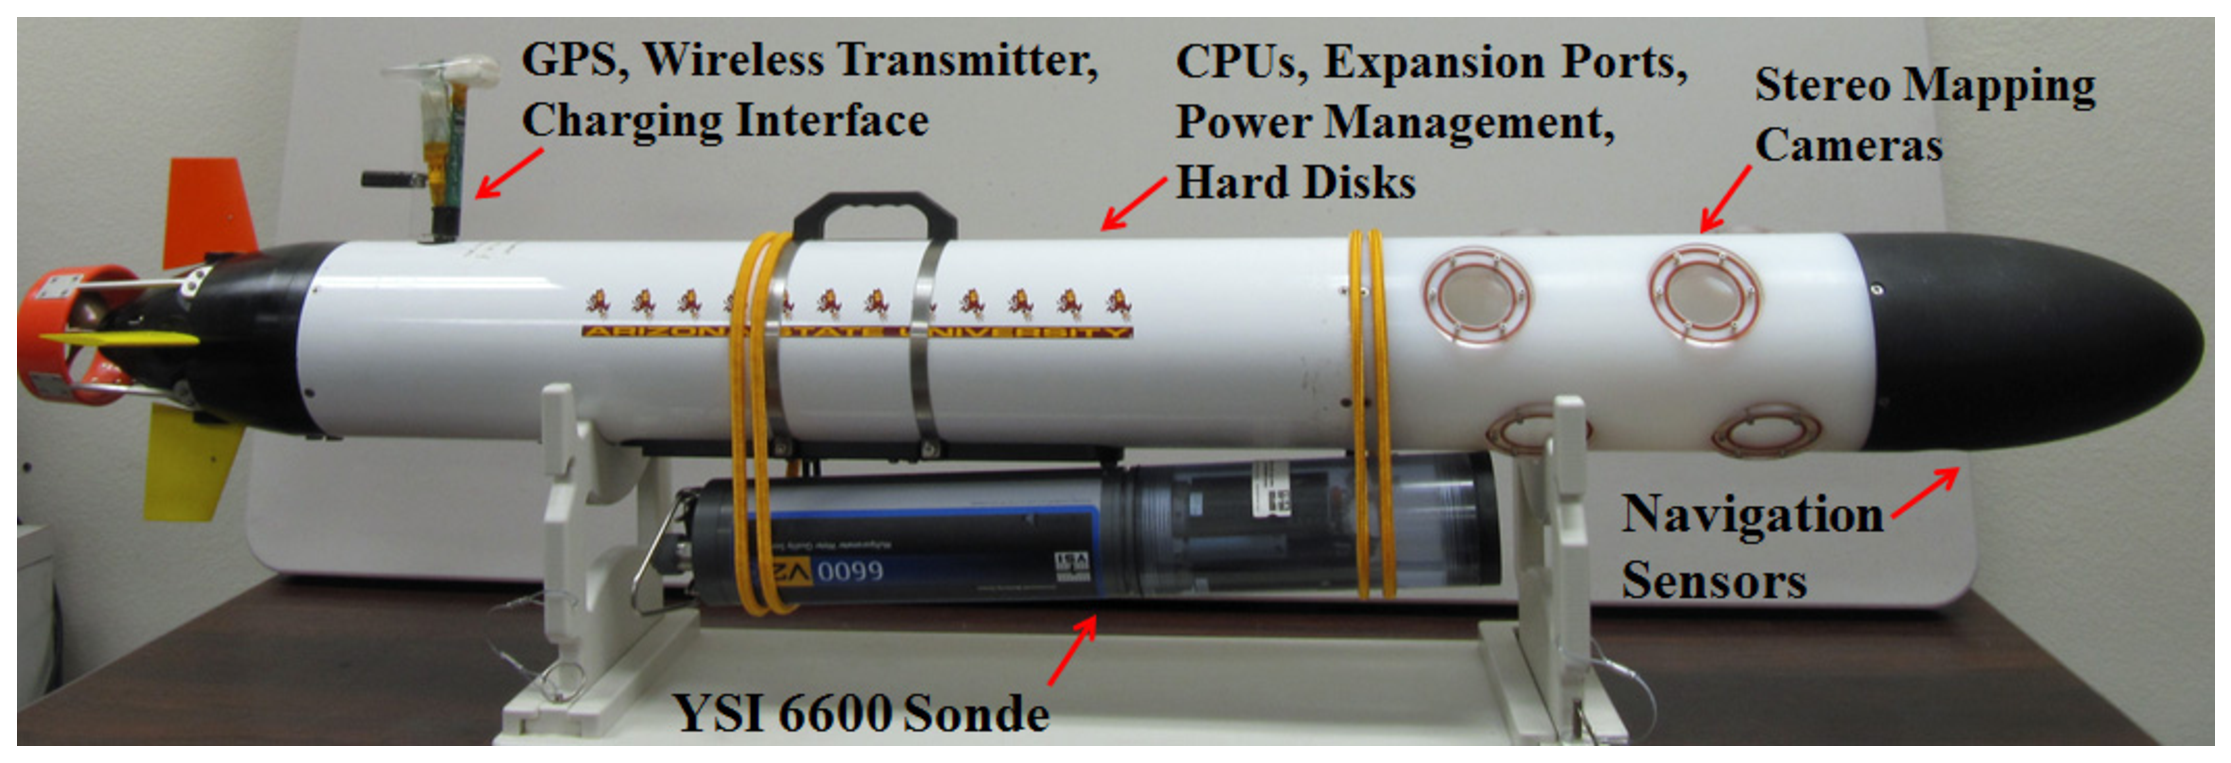
\includegraphics[width=\columnwidth, scale= 1.0]{figs/iverDescription1} %width=\columnwidth, scale= 1.0
        \caption{IVER: AUV testbed used during the autonomous sampling experiments presented in this paper.}
        \label{fig:iver}
     \end{subfigure}
     
     \vspace{0.5cm}
     
     \begin{subfigure}[b]{0.30\textwidth}
    	\centering
        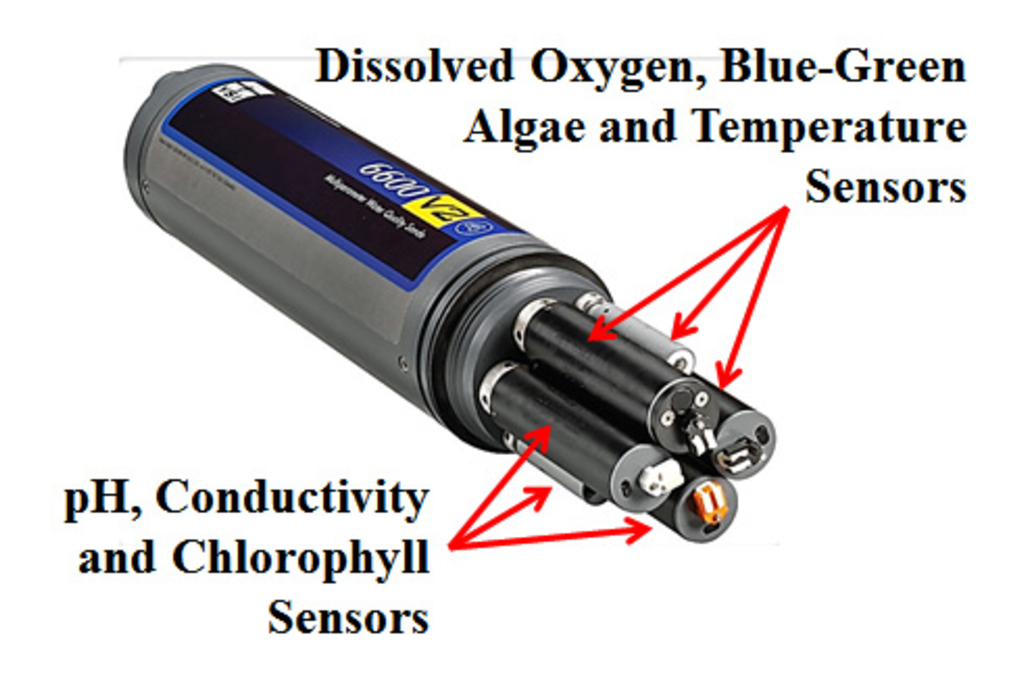
\includegraphics[width=\columnwidth, scale= 0.35]{figs/iverSonde1} %width=\columnwidth, scale= 1.0
        \caption{YSI Sonde.}
        \label{fig:ysiSonde}
     \end{subfigure}
\caption{Experimental Test-bed used during the autonomous sampling presented in this paper.}
\label{fig:testBed}
\end{figure}


\subsection{Environmental Sensor: Sonde YSI6000}
The instrumentation payload carried by our robotic platform was based on the YSI$6600$ sonde. 
This sonde measures temperature, turbidity, blue green algae (BGA), pH, dissolved oxygen and chlorophyll simultaneously. Standard measurement ranges for each of its sensors are summarized in Table \ref{tab:ysiSonde}. 

The sonde has a diameter of $8.9$[cm], a length of $54.9$[cm], and a weight of $3.18$[kg]. It is powered by $8$C-size alkaline batteries, it can operate between $-5$[\textcelsius] to $+50$[\textcelsius].

\begin{table}%[h!]
  \begin{center}
  	\caption{Characteristics of the Instruments on the YSI Sonde}
  	\label{tab:ysiSonde}
    \begin{tabular}{|m{2cm}|m{2.5cm}|m{2cm}|}
    	\hline
  		\bf{Sensor} & \bf{Range} & \bf{Resolution} \\
  		\hline
  		\hline
    	Optical Dissolved Oxygen & 0$\sim$50[mg/L] & 0.01[mg/L] \\
    	\hline
    	Conductivity & 0$\sim$100[mS/cm] & 0.001$\sim$0.1[mS/cm] \\
    	\hline
    	Temperature	 & -5$\sim$+50[\textcelsius] & 0.01[\textcelsius] \\
    	\hline
    	pH & 0$\sim$14[units] & 0.01[unit] \\
    	\hline
   		Turbidity & 0$\sim$1000[NTU] & 0.1[NTU] \\
   		\hline
    	Blue-Green Algae (BGA) & 0$\sim$280,000[cells/mL] & 1[cells/mL] \\
    	\hline
    	Chlorophyll & 0$\sim$400[\textmu g/L] & 0.1[\textmu g/L] \\
   		\hline
    \end{tabular}
  \end{center}
\end{table}



\subsection{Experimental Scenarios}
In order to observe possible changes over time and space in the quality of water of a large reservoir, we selected Lake Pleasant, Arizona as the location for our experiments.
Lake Pleasant is an artificial lake created in 1927 to provide the entire Phoenix area with a constant supply of potable water.
  
To observe changes over time, three different sets of experiments were carried out on 2010, 2011, and 2012. 
Each of these experiments were done during different seasons: Fall (2010), Summer (2011), and Winter (2012).
To understand if there are changes in the quality of the water at different locations in the same body of water, all of the experiments were performed in locations close to each other. 
The first two sets of experiments (Fall 2010 and Summer 2011) had a small overlap among them. 

An example of a sampled area and the sampling pattern made by our AUV platform is shown in Figure \ref{fig:samplingOverGoogleEarth} and Figure \ref{fig:samplingLocations}, respectively.
The approximate coordinates of the sampling location are $33$\textdegree $51' 55.66"$ N and $112$\textdegree$17' 45.01"$ W. 
In this particular experiment, the AUV collected 2258 samples over an area of approximately 70[m] x 100[m]. From this area, a subset of the samples from 30-70[m] northing and 30-70[m] easting was selected, given that this region contained the highest density of samples.

\begin{figure}[t]
\centering
	\begin{subfigure}[t]{0.35\textwidth}
	\centering
		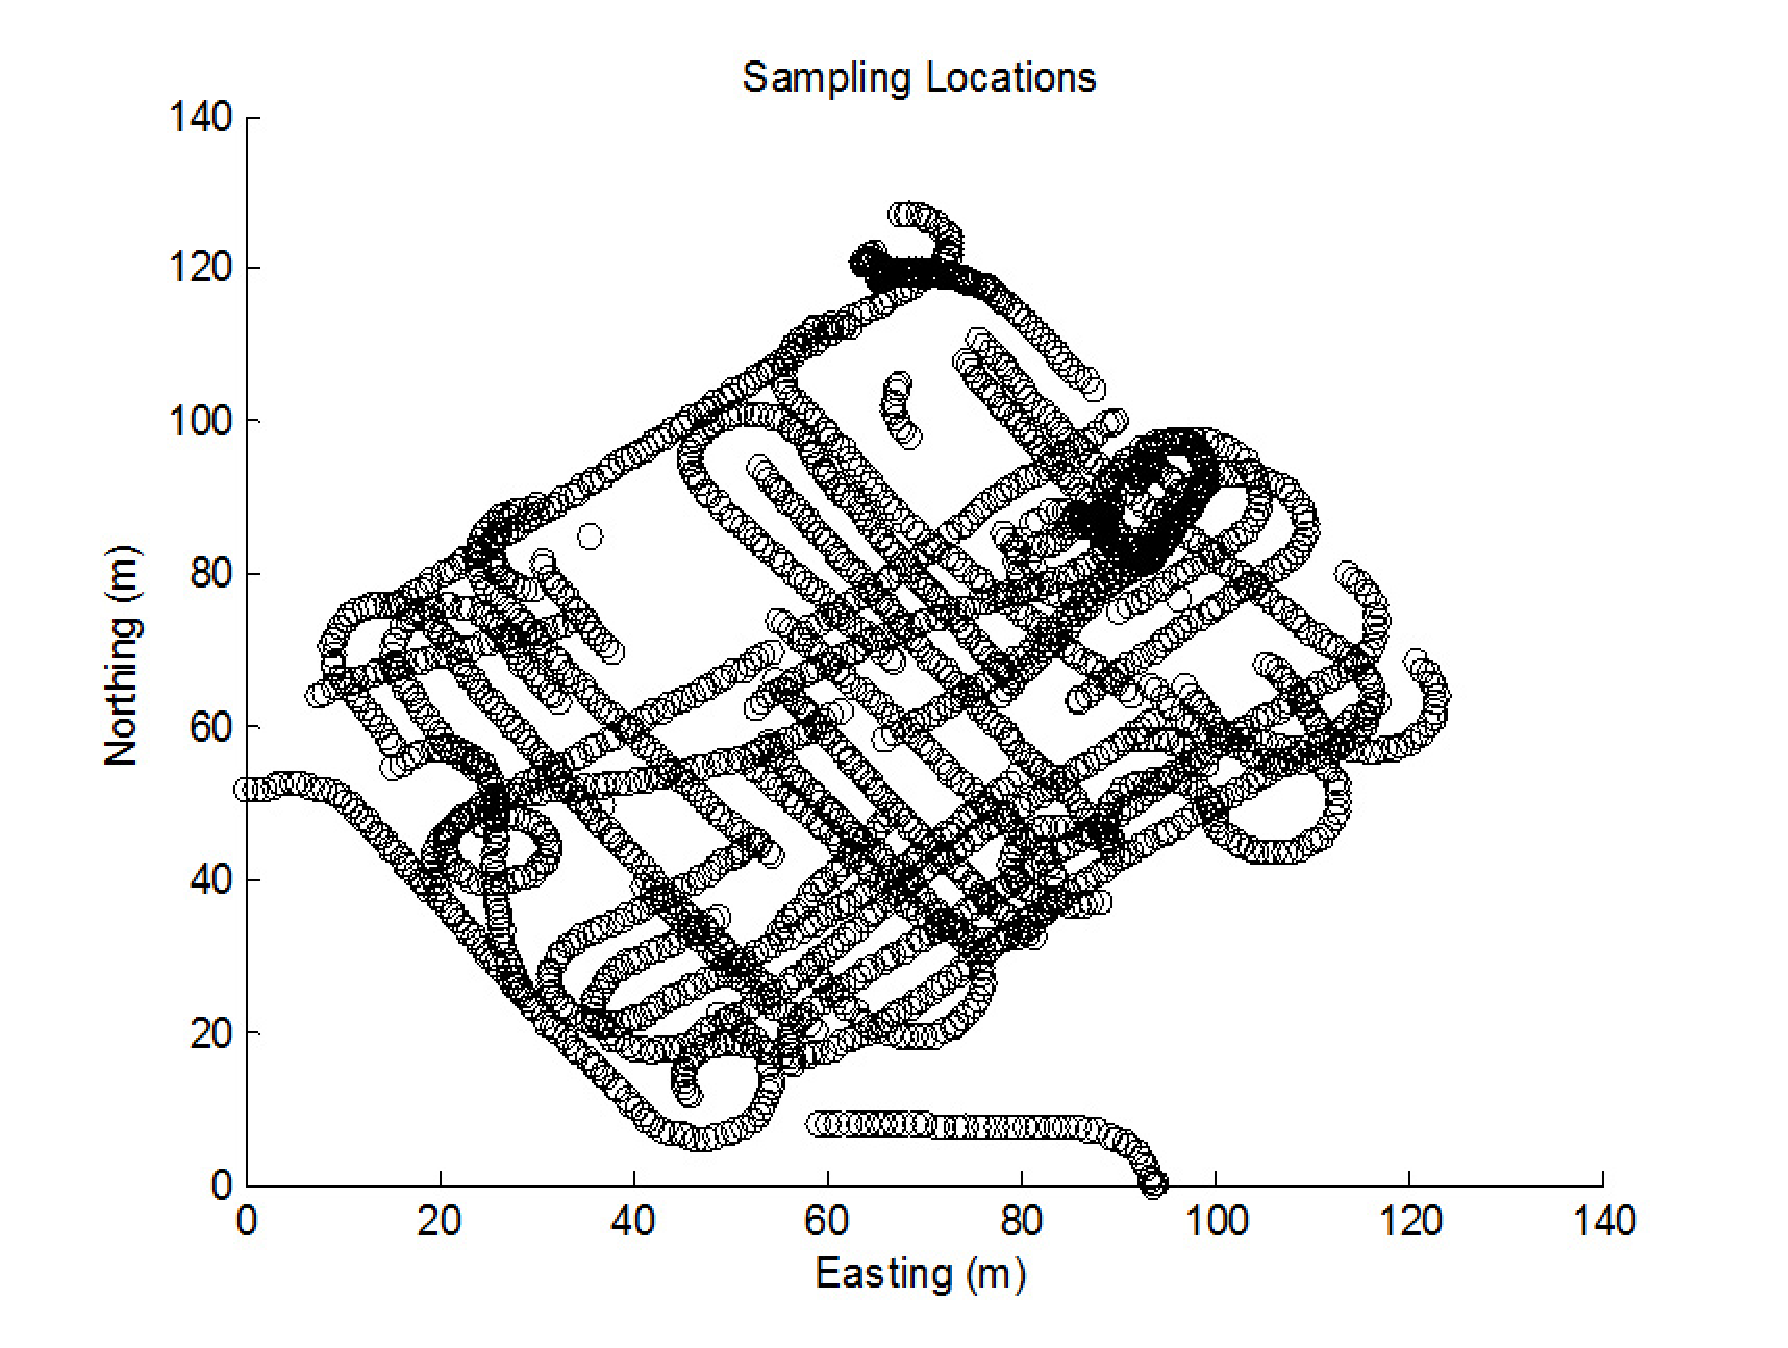
\includegraphics[width=\columnwidth, scale= 0.25]{figs/samplingLocations}
	\caption{Representation of the Sampling Locations.}
	\label{fig:samplingLocations}
	\end{subfigure}
	
	\vspace{0.5cm}
	
	\begin{subfigure}[t]{0.35\textwidth}
	\centering
		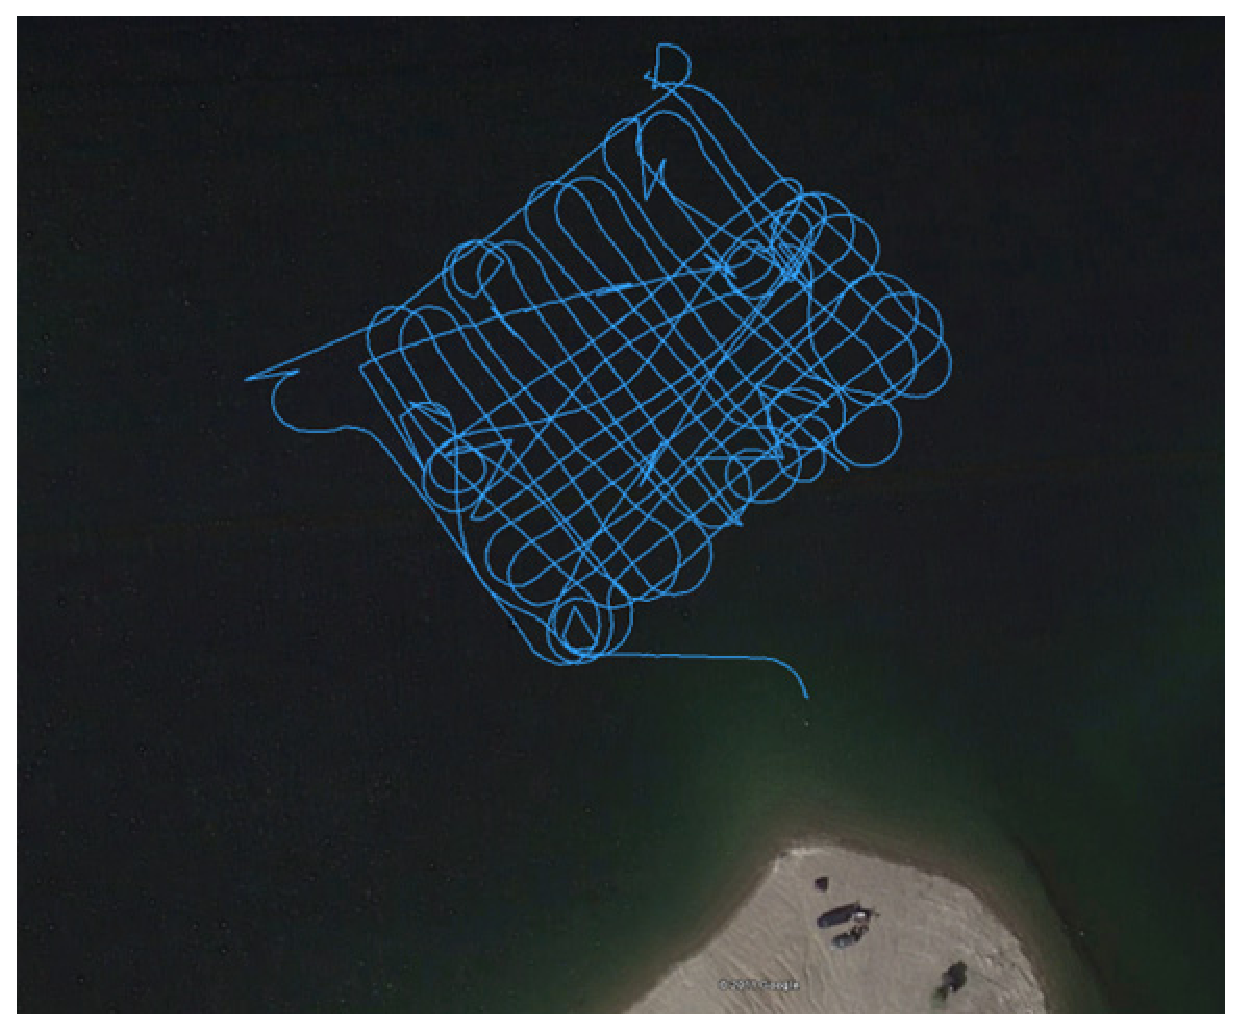
\includegraphics[width=\columnwidth, scale= 0.25]{figs/samplingOverGoogleEarth}
	\caption{Sampling Path at Lake Pleasant.}
	\label{fig:samplingOverGoogleEarth}
	\end{subfigure}
\end{figure}


%%%%%%%%%%%%%%%%%%%%%%%%%%%%%%%%%%%%%%%%%%%%%%%%%%%%%%%%%%%%%%%%
\section{Experimental Sampling Path Strategies}
Planning schemes require a priori knowledge of the environment or real time sensing and data feedback. 
There are many AUV deployments scenarios where there is a lack of a priori data on the environment, and the AUV is equipped with sensors that do not provide real time data (such as taking physical water samples) \cite{stoker:exploration}. 
Therefore, in many real world deployments, the paths chosen are often simple lawnmower patterns that may or may not be optimal for the situation they are being utilized \cite{forrest:investigation}, \cite{stoker:exploration}. 
The evaluation conducted in this paper is targeted at looking at autonomous underwater vehicle path planning from an experimental field scientist�s data sampling perspective. 
The goal is to comparatively evaluate various sampling path strategies using a cost-evaluation function that can optimize multiple parameters. 
These results from this evaluation will aid choosing the best sampling path strategy for unknown scalar fields, with no real time data feedback.

\subsection{Experimental Approach}
The evaluation consisted of conducting AUV sampling paths over various scalar fields to generate estimations of those scalar fields, and the energy consumption of the sampling path taken. 
Each of the simulated sampling paths and their corresponding scalar field estimation and energy consumption are then used as inputs for a cost-evaluation function that is used to comparatively determine the optimal sampling path.

\subsubsection{Assumptions}
\label{subsubsec:initAssump} 
The following assumptions are made:
\begin{itemize}
    \item[1)] The simulated AUV travels at a constant velocity and is capable of navigating to the desired sampling locations.
    \item[2)] The vehicle�s total energy consumption is based upon the total distance it travels, and the total angle it turns.
    \item[3)] The underlying scalar field being sampled has little or no temporal variation while being sampled.
    \item[4)] There is no real-time access to the sampled data; the samples can only be accessed offline.
  \end{itemize}

\subsubsection{Sampling Strategies}
The two main sampling strategy types that are evaluated are systematic sampling, and stratified random sampling.  
Systematic sampling is defined as sampling from an area of interest at regularly spaced intervals. 
Prior research has shown that having equilateral sampling grids is only optimal when the scalar field variation is isotropic \cite{mcbratney:exploration}. 
Therefore stratified random sampling was chosen as an additional sampling method to be comparatively evaluated. 
Stratified random sampling is conducted by splitting the desired sampling area into grid of equal sized sub-areas, in which samples are chosen from a random location in each sub-area. 
Stratified random sampling often produces a weighted mean with less variability than a standard random sampling. 
For each type of sampling strategy, lawn mower and spiral path patterns are evaluated. 
Both are simple path patterns which are commonly used for surveying. 
Example paths of the four sampling strategies are shown in Figure \ref{fig:samplingPatterns}.

\begin{figure*}[t]
	\begin{subfigure}[t]{\columnwidth}
    	\centering
        \includegraphics[scale= 0.30]{figs/lawn_path_evenPlot} %width=\columnwidth, scale= 1.0
        \caption{Even lawn mown}
        \label{fig:lawn_path_evenPlot}
     \end{subfigure}
     ~
     \begin{subfigure}[t]{\columnwidth}
    	\centering
        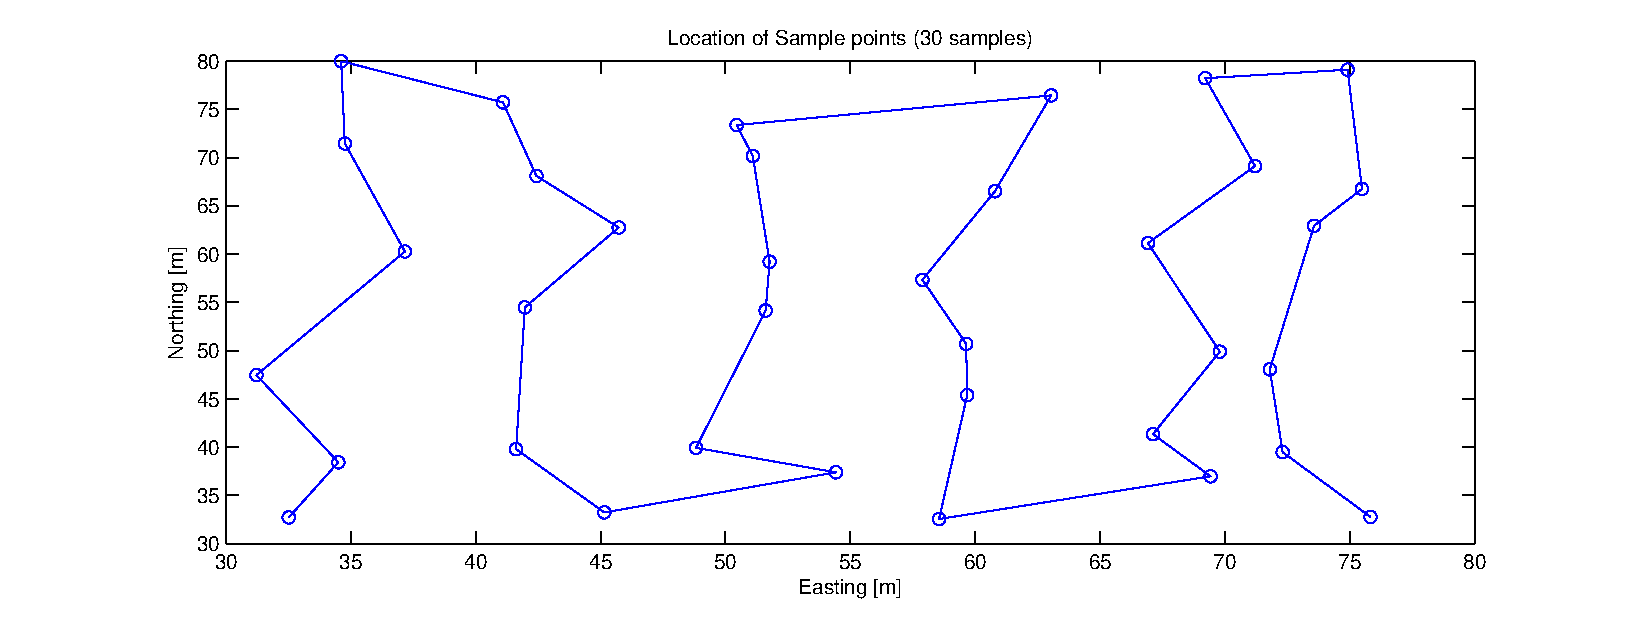
\includegraphics[scale= 0.30]{figs/lawn_pathPlot}
        \caption{Random lawn mown}
        \label{fig:lawn_pathPlot}
     \end{subfigure}

    \begin{subfigure}[b]{\columnwidth}
    	\centering
        \includegraphics[scale= 0.30]{figs/Spiral_path_evenv2Plot}
        \caption{Even spiral}
        \label{fig:Spiral_path_evenv2Plot}
     \end{subfigure}
     ~
     \begin{subfigure}[b]{\columnwidth}
    	\centering
        \includegraphics[scale= 0.30]{figs/Spiral_path_v2Plot}
        \caption{Random spiral}
        \label{fig:Spiral_path_v2Plot}
     \end{subfigure}
 \caption{Examples of the four evaluated sampling patterns}
 \label{fig:samplingPatterns}
\end{figure*}


\subsubsection{Underlying Scalar Field Data}
The underlying scalar field was represented with both real world and simulated data. 
The goal was to utilize enough scalar field data to be representative of many scalar field distributions commonly seen in real world data sets. 
Thus, six different underlying scalar fields were generated and collected for the purposes of this evaluation and are shown in Figure \ref{fig:underScalarFields}. 
The data sets derived from real world data consisted of a turbidity data set representing multi-modal data, a chlorophyll data set representing high anisotropy and variance, and a blue green algae cell count data set representing moderate anisotropy data with a high degree of spatial variance. 
The first simulated data set was a linearly varying distribution representing isotropic data. 
The second simulated data set was a normal distribution that represented moderately anisotropic data. 
The third and final simulated data set was a bi-modal normal distribution that represented moderate-variance anisotropic data.

\begin{figure*}[t]
	\begin{subfigure}[t]{0.3\textwidth}
    	\centering
        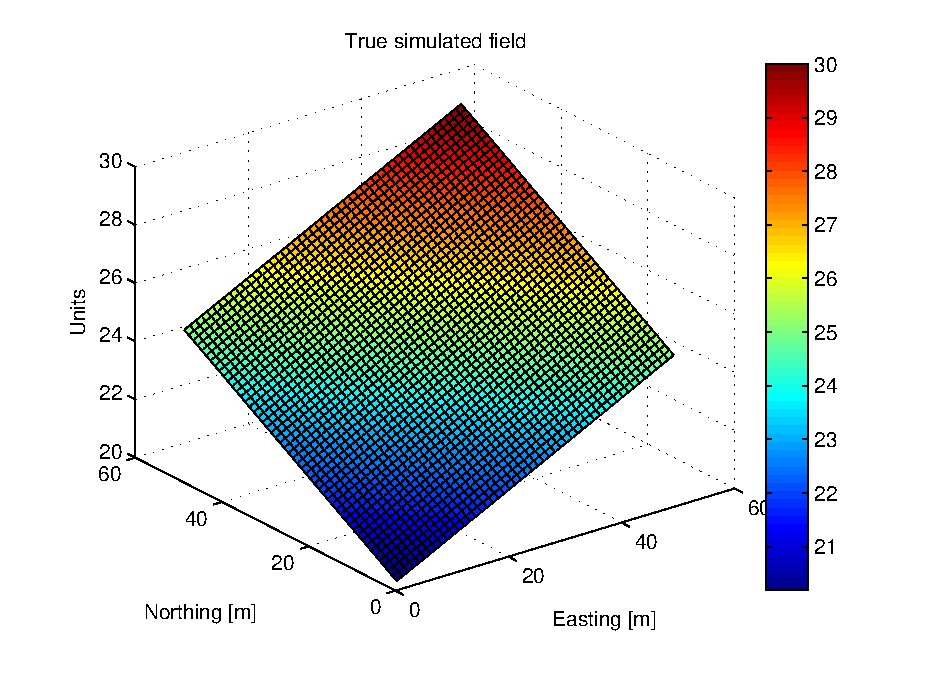
\includegraphics[scale= 0.30]{figs/Isotropic_spiral_even_8x7_true} %width=\columnwidth, scale= 1.0
        \caption{Isotropic}
        \label{fig:Isotropic_spiral_even_8x7_true}
     \end{subfigure}
     ~
     \begin{subfigure}[t]{0.3\textwidth}
    	\centering
        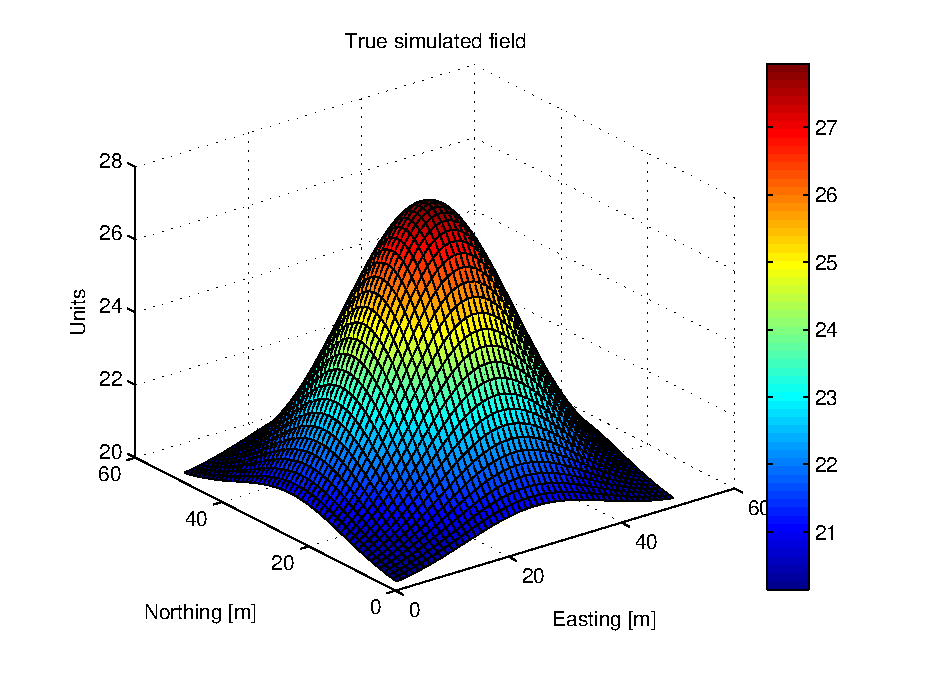
\includegraphics[scale= 0.30]{figs/Anisotropic1_spiral_even_8x7_true}
        \caption{Anisotropic 1}
        \label{fig:Anisotropic1_spiral_even_8x7_true}
     \end{subfigure}
     ~
	\begin{subfigure}[t]{0.3\textwidth}
    	\centering
        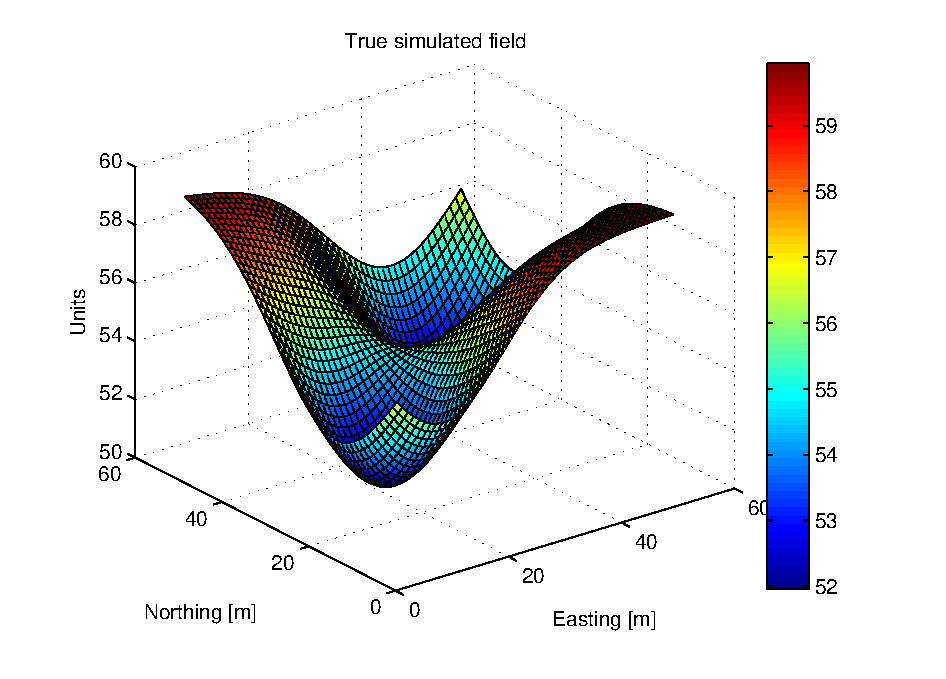
\includegraphics[scale= 0.30]{figs/Anisotropic4_spiral_even_12x10_true}
        \caption{Anisotropic 2}
        \label{fig:Anisotropic4_spiral_even_12x10_true}
     \end{subfigure}
     
     \vspace{0.5cm}
     
     \begin{subfigure}[b]{0.3\textwidth}
    	\centering
        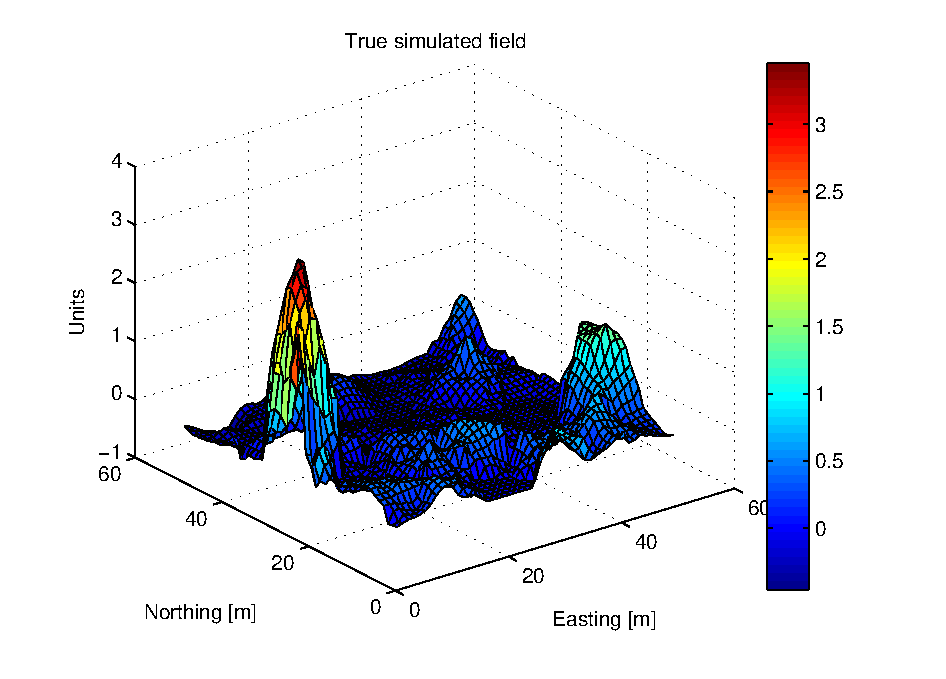
\includegraphics[scale= 0.30]{figs/Turbidity_spiral_even_10x9_true}
        \caption{Turbidity}
        \label{fig:Turbidity_spiral_even_10x9_true}
     \end{subfigure}
	 ~
     \begin{subfigure}[b]{0.3\textwidth}
    	\centering
        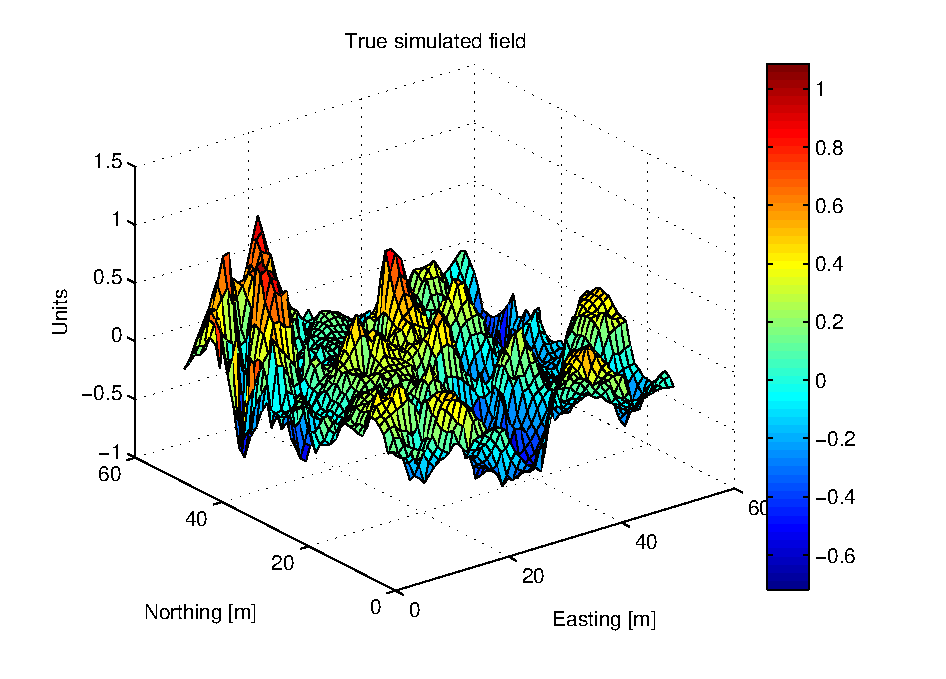
\includegraphics[scale= 0.30]{figs/Cholorophyll_spiral_rand_9x8_true}
        \caption{Cholorophyll}
        \label{fig:Cholorophyll_spiral_rand_9x8_true}
     \end{subfigure}
     ~
     \begin{subfigure}[b]{0.3\textwidth}
    	\centering
        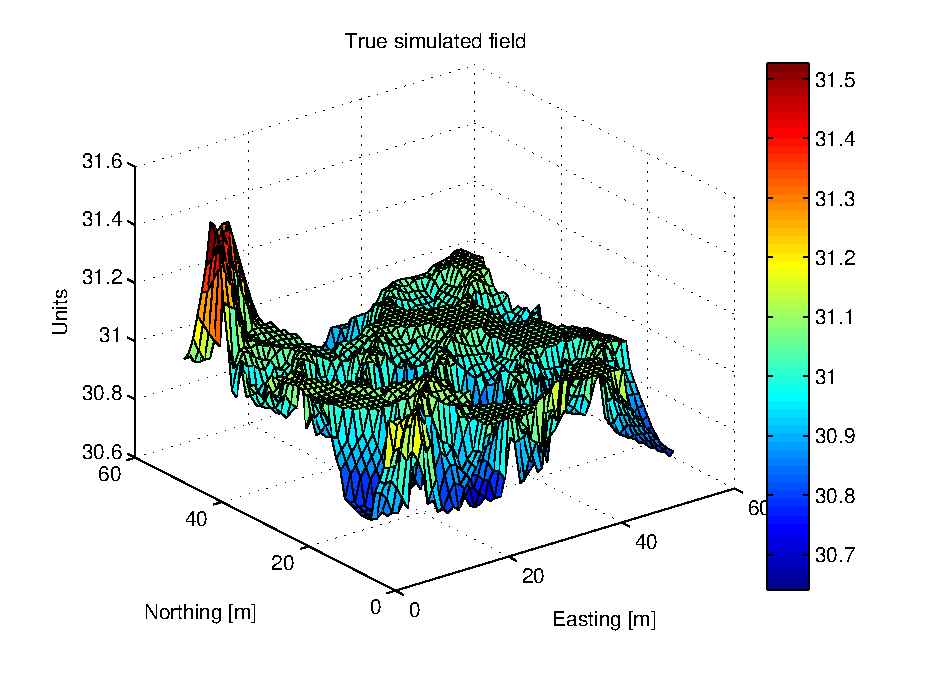
\includegraphics[scale= 0.30]{figs/BlueGreenAlgae_lawn_rand_12x10_true}
        \caption{Blue Green Algae}
        \label{fig:BlueGreenAlgae_lawn_rand_12x10_true}
     \end{subfigure}
 \caption{Examples of the four evaluated sampling patterns}
 \label{fig:underScalarFields}
\end{figure*}

\subsection{Evaluation Methods}

\subsubsection{Estimation Evaluation}
Once a sampling path has been generated, it is then used to sample the underlying scalar field. 
With those samples, an estimation of the underlying scalar field is generated through ordinary Kriging. 
Kriging is a form of linear least squares estimation that interpolates the value of a location upon a scalar field from known values at nearby locations, which in this case are the sampled locations \cite{delhomme:kriging}.
Ordinary Kriging is a specific type of Kriging that assumes that the experimental variogram can be constructed, and that the mean of the scalar field being estimated is unknown but constant. 
$Z$ represents the underlying scalar field, thus the Kriging estimation of the scalar field at any location is the weighted average of observed values. 
This is represented through the following equation (\ref{eq:scalarField}). 

\begin{equation}
z(x_0) = \Sigma^n_{i=1} w_i z(x_i)
\label{eq:scalarField}
\end{equation}

The estimation variance of $z(x_0)$ is given by

\begin{equation}
\sigma^2_k = 2 \Sigma^n_{i=1} w_i \gamma(x_i, x_0) - \Sigma^n_{j=1} w_i w_j \gamma(x_i, x_j)
\label{eq:estimVar}
\end{equation}

where $\gamma(x_i, x_0)$ is the variogram of $x_i$ and $x_0$. 
The weights $w_i(x)$ are chosen such that tehy fulfull the unbiasedness condition (they all sum to $1$), and also minimize the estimation variance.
Thus, the weights are determined through the equation (\ref{eq:weights})

\begin{equation}
\Sigma^n_{j=1} w_j \gamma(x_i, x_j) + \psi = \gamma(x_i, x_0)
\label{eq:weights}
\end{equation}

where $\gamma$ is the Lagrance parameter associated with the minimization.
Once the Kriging estimation was generated, it accuracy is evaluated through the computation of its integrated mean square error (IMSE) with respect to the underlying scalar field.


\subsubsection{Energy Consumption Evaluation}

The energy consumed by the vehicle travelling along the sampling path was computed through the use of a simple energy consumption model.
The model has two input parameters; the distance travelled, and the total angle turned.
Since it is assumed that the vehicle is travelling straight at a constant velocity, it is extrapolated that the vehicle consumes its stored energy at a constant rate.
An autonomous underwater vehicle may also experience in increase in energy consumption while turning.
This additional increase may be nominal or significant, depending on the design of the vehicle.
Therefore the model takes the additional energy consumption while turning into consideration through the use of a constant multiplier for the total turn angle.
The energy consumption equation is modeled through the following equation \ref{eq:energyConsumption}:

\begin{equation}
E(d, \theta) = d + k_\theta
\label{eq:energyConsumption}
\end{equation}

For this equation, $d$ and $\theta$ respectively represent the total distance of the sampling path, and the cumulative turn angle.
The constant $k_\theta$ is a constant multiplier that represents the increase in energy consumption while turning for a vehicle.
This weight is better understood through the following relationship,

\begin{equation}
k_\theta = \frac{d_t}{90^o}
\label{eq:weightK}
\end{equation}

This relation defined as such; for each right angle turn taken, an additional energy penalty of travelling a straight distance $d_t$ is added.

\subsubsection{Cost-Evaluation Function}
The cost-evaluation function is a general evaluation method that allows for quantitative comparative analysis for multiple input parameters. 
It normalizes and then assigns each input parameter a weight, allowing for the function to prioritize each parameter in respect to one another. 
These weights must all sum to one. 
In the case of this evaluation, we are investigating which sampling strategy is optimal for both estimation error and energy consumption. 
Therefore the parameters that were selected to be inputs for the cost-evaluation function were the total distance travelled  $d$, the total energy consumed $E$, and the IMSE for the specific sampling path taken $\epsilon$.  
Our proposed cost-evaluation function is as follows in equation \ref{eq:costFunction},

\begin{equation}
E(p) = \Sigma_{i=p} W_d N_d d_i + W_E N_E E_i + W_\epsilon N_\epsilon \epsilon_i
\label{eq:costFunction}
\end{equation}

where $W_d$, $W_E$, and $W_\epsilon$, are the weighted factors that provide specific priorities between the total distance travelled, the total energy consumed, and the IMSE for the sampling path taken.  
$N_d$, $N_E$, and $N_\epsilon$ are normalization factors assigned constant values to normalize each of their corresponding parameters and eliminate their dimensions.

\subsection{Experimental Results}

\subsubsection{Underlying Scalar Field Data Generation}
The six different scalar fields used in this evaluation were either generated from simulated equations, or from a real world dataset. 
The isotropic scalar field used for this evaluation was generated by the following equation.

\begin{equation}
I(x, y) = \frac{x+y}{0.1} + 20
\label{eq:isoScalarField}
\end{equation}

The first simulated anisotropic scalar field was generated by using a standard normal distribution and then scaling it by a factor of 50 and offseting by $+20$. 
The multi-modal anisotropic field was generated by simply adding together two equally scaled inverted normal distributions with differing $x-y$ locations for their means. 
The real world dataset used for generating the turbidity, chlorophyll and blue green algae scalar fields was created by sampling a local freshwater lake with an autonomous underwater vehicle carrying a water quality monitoring sonde. 
The contiguous underlying scalar field was then generated by interpolating the samples using ordinary kriging.

%The AUV to used to collect the samples was a heavily modified OceanServer IVER2 platform, which carries a YSI 6600V2 water quality monitoring sonde. 
%The sonde sampled the in-situ turbidity, cholorophyll, and blue green algae, among a variety of other measurements.

\subsubsection{Estimation Error Computation}
To compute the estimation error, an estimate of the underlying scalar field was first generated for each of the sampling strategy types. 
These estimates were generated across varying sampling grid sizes in order to characterize a range of sampling densities from low to high. 
The sampling grid dimensions and total sample size are listed in Table \ref{tab:sampleDistr}.

\begin{table}%[h!]
  \begin{center}
  	\label{tab:sampleDistr}
  	\caption{Sample Distribution Grid Sizes}
    \begin{tabular}{|ccc|}
    	%\hline
    	\hline
  		\bf{Grid} & \bf{Dimensions} &  \\
  		\it{Size in X} & \it{Size in Y} & \bf{Sample Count}\\
  		\hline
  		\hline
    	5 & 4 & 20 \\
    	\hline
    	6 & 5 & 30 \\
    	\hline
    	7 & 6 & 42 \\
    	\hline
    	8 & 7 & 56 \\
    	\hline
   		9 & 8 & 72 \\
   		\hline
    	10 & 9 & 90 \\
    	\hline
    	12 & 10 & 120 \\
   		\hline
    \end{tabular}
  \end{center}
\end{table}

The IMSE for each of the stratified random sampling strategy based estimations was the average of fifteen iterations, in order to generate a stable value. 
The systematic sampling estimation was iterated five times at five separate evenly distributed path seeding locations to remove biasing in error results.
These seeding locations are shown in Figure \ref{fig:pathSeedingPositions}. 

\begin{figure}[htp]
	\centering
		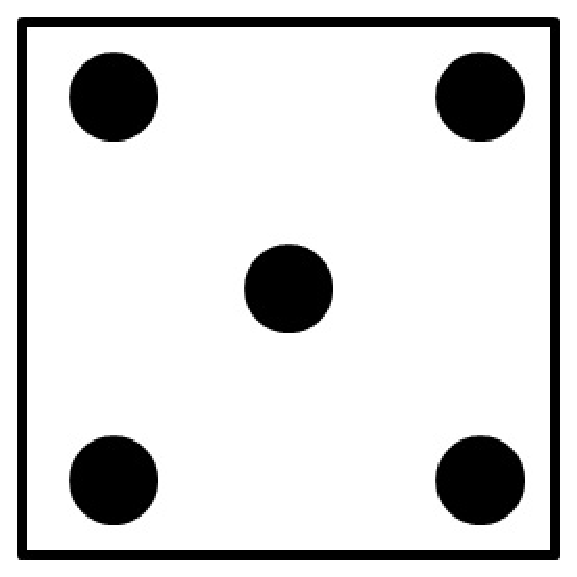
\includegraphics[width=0.10\textwidth]{figs/pathSeedingPositions}
	\caption{Systematic path seeding positions for averaging.}
	\label{fig:pathSeedingPositions}
\end{figure} 


\subsubsection{Estimation Error Result}
The IMSE error for each of the scalar varying from low (20 samples), moderate (56 samples) and high (120 samples) sampling density are displayed alongside one another in the Table II on the following page.

% \begin{table}
% 	\centering
% 	\begin{tabular}{|cccccccc|}
% 	\hline
% 	\bf{Sample Size} & \bf{Sampling Strategy} & \bf{Isotropic} & \bf{Anisotropic 1} & \bf{Anisotropic 2} & \bf{Turbidity} & \bf{Chlorophyll} & \bf{Blue Green Algae} \\
% 	\hline
% 	
% 	\end{tabular}
% 	\caption{Cost-Evaluation Function Outputs for Varying Scalar Fields and Sample Densities}
% \end{table}

\begin{figure*}
	\centering
	\begin{subfigure}[t]{0.35\textwidth}
		\centering
			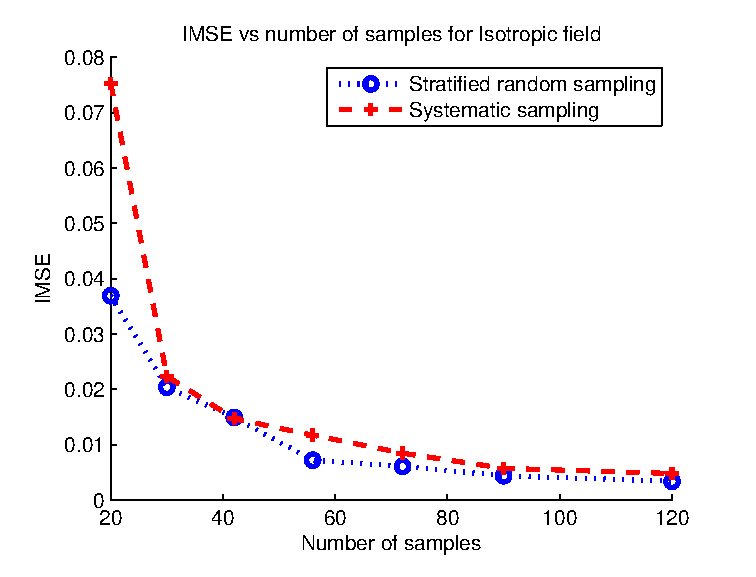
\includegraphics[width=\columnwidth, scale= 0.25]{figs/Isotropic_IMSE}
		\caption{Representation of the Sampling Locations.}
		\label{fig:samplingLocations}
	\end{subfigure}
	~
	\begin{subfigure}[t]{0.35\textwidth}
		\centering
			\includegraphics[width=\columnwidth, scale= 0.25]{figs/Anisotropic1_IMSE}
		\caption{Representation of the Sampling Locations.}
		\label{fig:samplingLocations}
	\end{subfigure}
	
	\vspace{0.5cm}
	
	\begin{subfigure}[t]{0.35\textwidth}
		\centering
			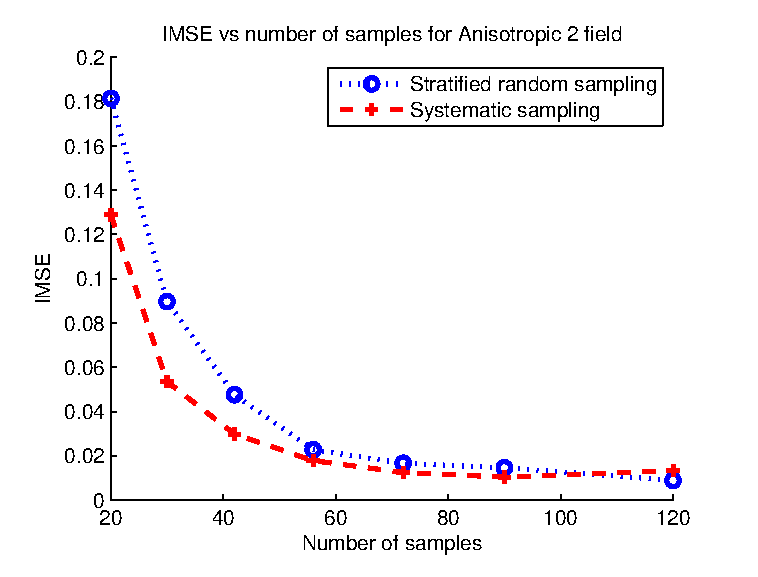
\includegraphics[width=\columnwidth, scale= 0.25]{figs/Anisotropic2_IMSE}
		\caption{Representation of the Sampling Locations.}
		\label{fig:samplingLocations}
	\end{subfigure}
	~
	\begin{subfigure}[t]{0.35\textwidth}
		\centering
			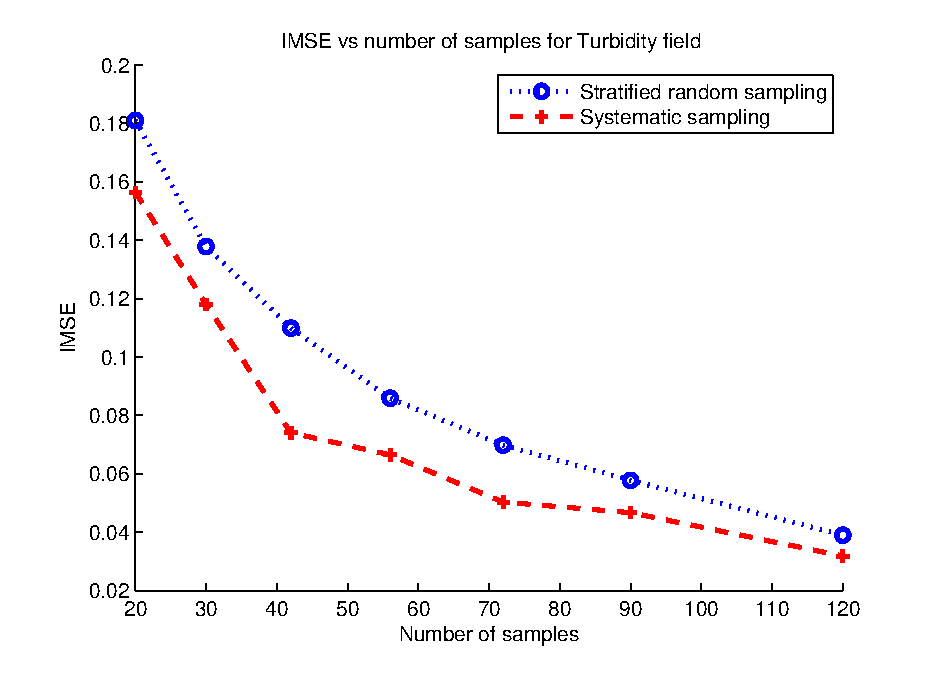
\includegraphics[width=\columnwidth, scale= 0.25]{figs/Turbidity_IMSE}
		\caption{Representation of the Sampling Locations.}
		\label{fig:samplingLocations}
	\end{subfigure}
	
	\vspace{0.5cm}
	
	\begin{subfigure}[t]{0.35\textwidth}
		\centering
			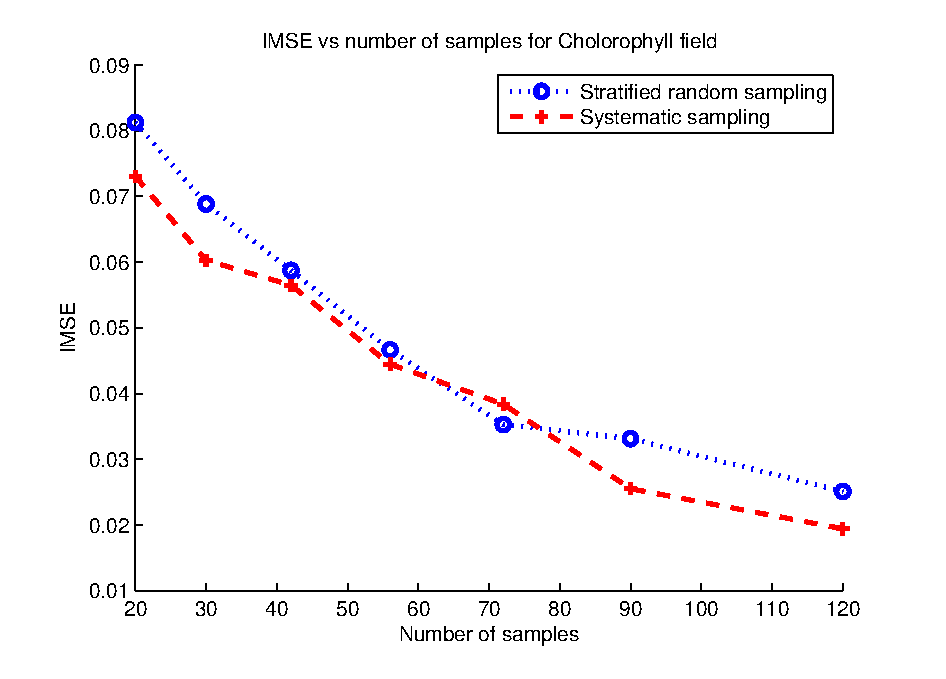
\includegraphics[width=\columnwidth, scale= 0.25]{figs/Cholorophyll_IMSE}
		\caption{Representation of the Sampling Locations.}
		\label{fig:samplingLocations}
	\end{subfigure}
	~
	\begin{subfigure}[t]{0.35\textwidth}
		\centering
			\includegraphics[width=\columnwidth, scale= 0.25]{figs/BlueGreenAlgae_IMSE}
		\caption{Representation of the Sampling Locations.}
		\label{fig:samplingLocations}
	\end{subfigure}
\end{figure*}

Through looking at the IMSE versus number of sample plots for the various underlying scalar fields, a number of correlations are apparent. 
Firstly, both strategies demonstrate a reduction in IMSE as the number of samples increases, as one would expect. 
Additionally, it is found that the systematic sampling strategy minimizes error for the real world data sets across all sampling densities. 
The stratified random sampling strategy minimizes error for the low variance isotropic and anisotropic 2 data sets. 
Finally, for the anisotropic 1 data set, the systematic sampling strategy significantly minimizes error for low sampling densities, and the stratified random sampling strategy minimizes error for moderate and high sampling densities.

\subsubsection{Energy Consumption Computation}
The energy consumption of each of the sampling path patterns was computed using equation \ref{eq:energyConsumption}. 
First, the distance and total angle turned was computed for each of the sampling path types through the range of sampling densities shown in Table I.  
For each of the stratified random sampling paths, the total distance travelled and total cumulative angle turned was computed as the averages of 50 iterations of each sample grid size. 
Finally equation \ref{eq:energyConsumption} was applied using $k_\theta$ values from a range of 0 to 2. 
This range characterizes vehicles for which a $90^o$ turn correlates to consuming the energy equivalent to travelling an additional distance of 0[m] to 2[m].

\subsubsection{Energy Consumption Results}
The average total energy consumption versus the $k_\theta$ for each of the sampling path strategies is shown in Fig. 9. 
The resulting total energy versus $k_\theta$ plots were then fitted to linear equations to quantify their relationship. 
The resulting energy consumption model equations for each of the sampling path strategies are shown below in Table III.

It is shown in the energy consumption model equations, that the even spiral sampling path strategy is the most energy efficient, and through viewing Figure 9, it is easily apparent.

\subsubsection{Cost-Evaluation Computation}

The cost-evaluation function was computed with the all the weighted factors set equal to $1/3$, thus weighting all of the evaluation parameters equally. 
To compute the energy for each sampling path, $k_\theta$ was set to $0.1$. 
The function was applied to each of the sampling strategies for all the underlying scalar fields, at 20, 56, and 120 samples. 
This was done such that a comparative analysis of each of the sampling strategies at low, moderate and high sampling densities could be conducted. 

\subsubsection{Cost-Evaluation Results}
The results of the cost-evaluation are listed in Table IV. 
For a low sampling density the systematic spiral sampling method is optimal for all of the data sets except for the isotropic scalar field. 
For a moderate sampling density the systematic spiral strategy is optimal for the anisotropic 1, turbidity, and chlorophyll scalar fields. 
The random lawnmower and random spiral strategies are optimal for the anisotropic 2 and isotropic scalar fields respectively. 
Finally, for a high sample density the random spiral strategy is optimal for the isotropic and both of the anisotropic scalar fields. 
The systematic spiral strategy was found to be optimal for the turbidity, cholorophyll and blue green algae scalar fields. 
The strategy that was optimal for the most types of scalar fields and densities was found to be the systematic spiral strategy. 
In general, a spiral path strategy was found to be the optimal in almost all of the cases. 

\subsection{Discussion}
The results from this cost-evaluation are specific to the weights given to the cost-evaluation function. 
However these results do provide insight into which sampling strategies are optimal for different types of scalar fields, given the assumption that distance travelled, total energy consumption and IMSE are considered equal factors in optimality. 

For isotropic scalar fields, the random spiral sampling strategy was found to be the optimal sampling strategy for all sampling densities. 

It was found that in low variance scalar fields, such as the single/multi-modal anisotropic scalar fields used in this evaluation, the systematic spiral strategy is optimal for coarse sampling densities, and the random spiral strategy is optimal for high sampling densities.

In high variance scalar fields such as the turbidity, chlorophyll and blue green algae data sets, the systematic spiral strategy was optimal for almost every case.

\section{AUV Energy Dynamical Modelling}
\label{dynModel}

\subsection{Motivation}
Mobile robotics are key to facilitate and improve the automation of environmental sensing, however the length they can cover is limited by the amount of energy they carry with them.
%-----The rate at which the vehicle consumes its energy is related to the number of
In our experimental setting, the problem then depends on how the sampling patterns studied in this paper affect the amount of stored energy our platform holds onboard.
In previous studies \cite{ho:where}-\cite{ho:icra2012} we've relied on a simple approach to model the energy consumption of our robotic platform.
Using this simple model as a starting point, we have expanded it and considered a new approach to model the dynamic behavior of the AUV used in this research.


Although solving the kinematics and dynamics of a mobile robot and in this particular case of a torpedo-like AUV is a well understood task, its solution is highly dependent on parameters such as its physical characteristics and forces acting on the robot.
It is also time-consuming as it usually deals with large matrices and its computation is complex.
The approach we propose in this paper aims to simplify this procedure and to make it easier for non-roboticists to determine the dynamics of their robotic platform based on only the knowledge of the robot's inputs and outputs.
This method can be explained as describing what happens inside of a ``black box'' from which we can only see what gets in and what gets out.

\subsection{Dynamical Model}
Our approach consists of an estimation of the dynamical model of the robot based on the selection of two known inputs and one output from the data acquired.
The two inputs of the estimation were the velocity and the heading of the vehicle measured by the on-board GPS.
The data acquisition frequency was set to $2Hz$.
The output selected for the estimation of our model was the total power consumed by the vehicle during the sampling mission. 

By estimating the dynamical model of the robot, it is not required to assume that the vehicle is travelling straight at a constant velocity, thus there is no restriction with respect to the rate at which the vehicle consumes its stored energy.
An increase in the energy consumed by the vehicle while it turns may be nominal or significant, depending on the design of the vehicle.
The estimated model incorporates the possible effect in the increment in energy consumption a turning maneuver may represent by including the changes in the orientation of the vehicle.
The velocity of the vehicle (in knots), its heading (in degrees) and the corresponding power consumption (in Watts) measured by the instruments on-board are presented in Figure \ref{fig:inputsVsOutput}.

\begin{figure*}
	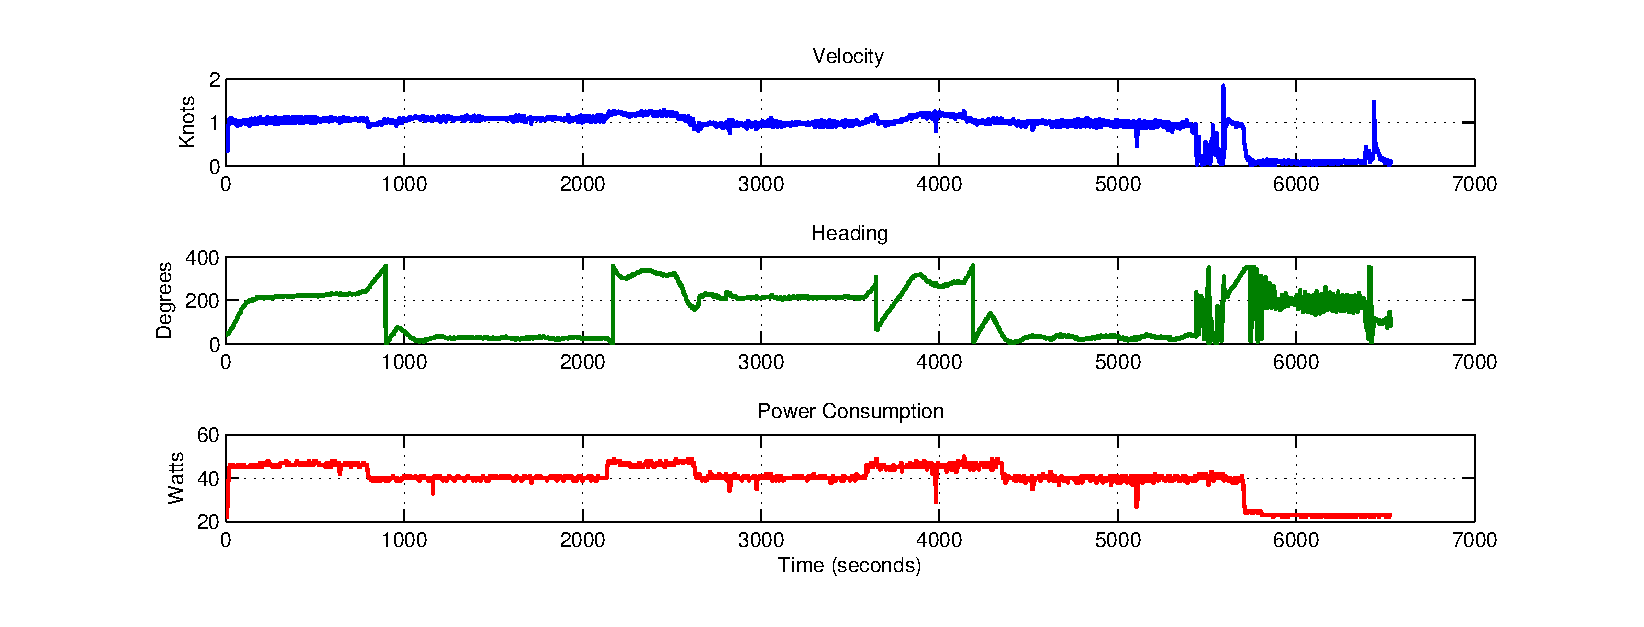
\includegraphics[width=\textwidth, scale= 0.10]{figs/inputsVsOutput.eps}
	\caption{Velocity, heading and power consumption used to estimate the vehicle's dynamical model.}
	\label{fig:inputsVsOutput}
\end{figure*}

We used two different methods to obtain our estimation and after comparing the one with the best fit to our validation data was selected.
One estimation method consisted of first calculating the state-space model using a sub-space method and later on refining the model by computing the prediction error estimate of the state-space model \cite{van:subspace}.
The second method was based on a combination of an Auto-Regressive eXogenous (ARX) and a Non-Linear ARX model estimator. REFERENCES HERE.

In order to estimate and validate the model, the estimation is based on half of the entire data set and it is later validated using the remaining half of the data set acquired by the vehicle's instruments.

\subsubsection{State-space estimation model}
In order to obtain the desired dynanical model, we first start by estimate a discrete-time state-space model using a sub-space method REFERENCE.
Later we apply an iterative prediction-error minization method to obtain the parameters of our estimate model.
The resulting dynamic model obtained from the estimation follows the standard state-space model convention as presented by equation \ref{eq:dynModel_1}:

\begin{equation}
 \left\{\begin{aligned}
        x(t + Ts)	&= Ax(t) + Bu(t) + Ke(t) \\
        y(t)	&= Cx(t) + Du(t) + e(t)
       \end{aligned}
       \right.
\label{eq:dynModel_1}
\end{equation}

where 
$ 
A = 
\bigl[
\begin{smallmatrix}
	0.99495		&	-0.069517 \\
	 -0.0032466	&	0.86892
\end{smallmatrix} 
\bigr]
$,
$ 
B = 
\bigl[
\begin{smallmatrix}
	0.021859	&	1.0813e^{-5} \\
    -0.039972	&	1.9386e^{-5}
\end{smallmatrix} 
\bigr]
$,
$ 
C = 
\bigl[
\begin{smallmatrix}
	126.37	& 6.4396
\end{smallmatrix} 
\bigr]
$,
$ 
D = 
\bigl[
\begin{smallmatrix}
	0 & 0
\end{smallmatrix} 
\bigr]
$, 
$ 
K = 
\bigl[
\begin{smallmatrix}
	0.0070135	\\
    0.0090162
\end{smallmatrix} 
\bigr]
$, and 
$ 
x(0) = 
\bigl[
\begin{smallmatrix}
	-0.14306\\
    -0.36083
\end{smallmatrix} 
\bigr]
$.

The resulting power based on the estimated dynamical model is compared against the half of the data set used to validate the model as shown in Figure \ref{fig:estVsMeaPwr}. 

\begin{figure}[htp]
	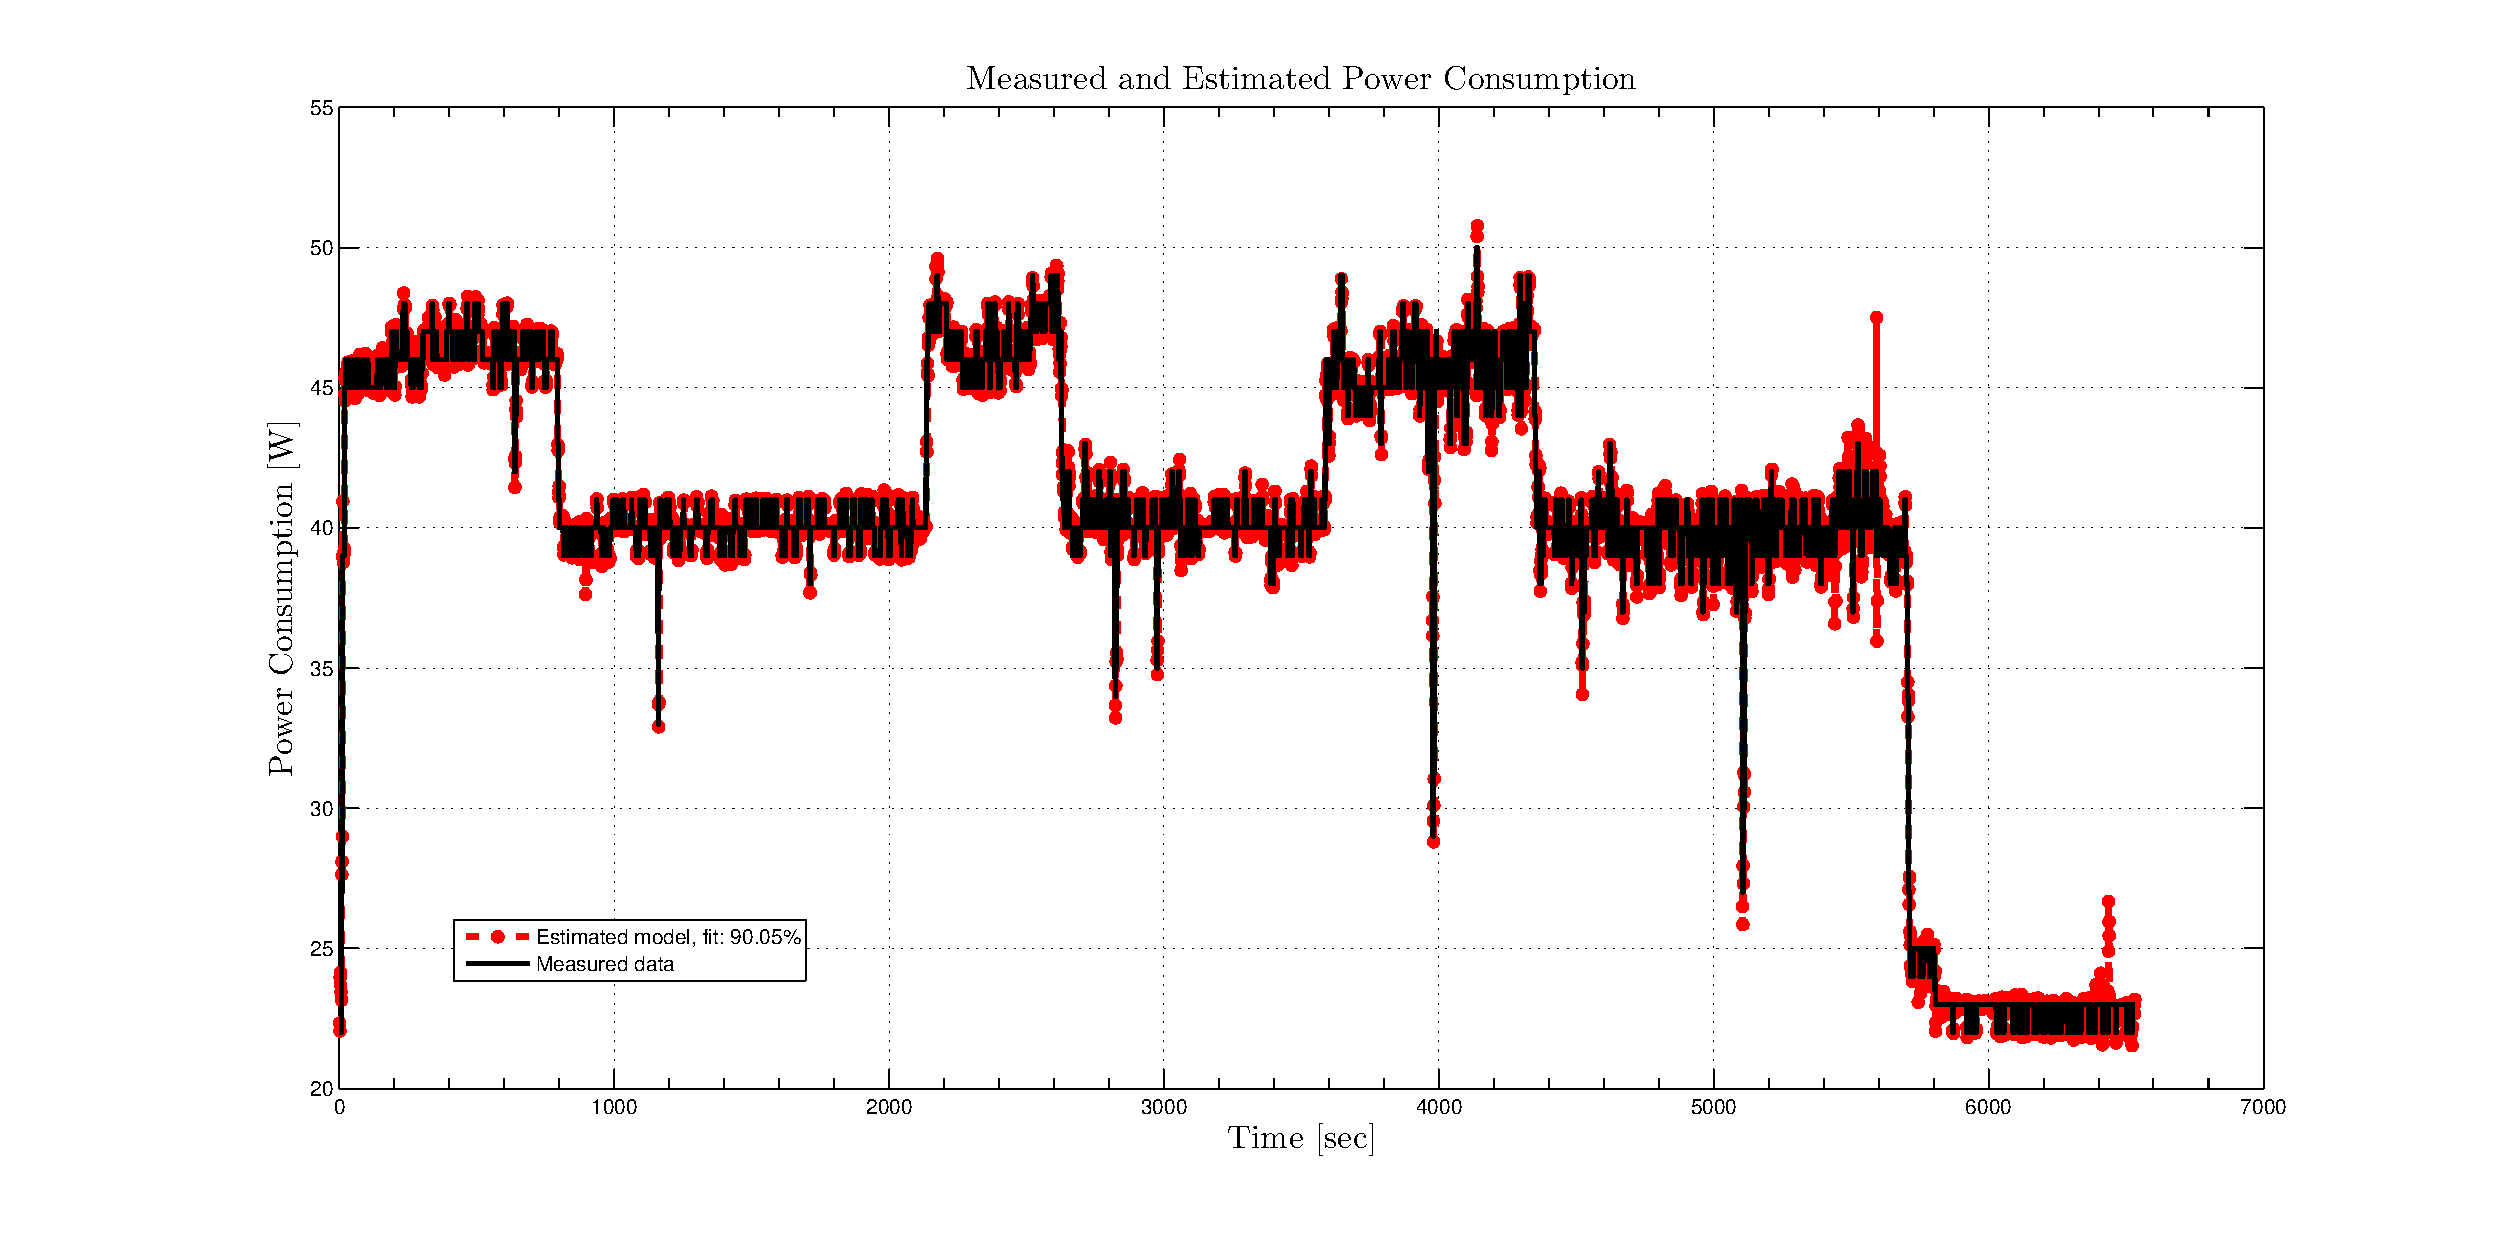
\includegraphics[width=\columnwidth, scale= 1.0]{figs/estimatedVsMeasuredPowerStateSpace_1}
	\caption{Estimated vs Measured Power Consumption using a State-space method.}
	\label{fig:estVsMeaPwr}
\end{figure}

\subsubsection{ARX and Nonlinear-ARX Estimation Model}
An alternative method to estimate the dynamical model of our robotic platform is based on a combination of an ARX and a nonlinear-ARX estimation.
We initially compute the parameters of the ARX model which are described in equation \ref{eq:arxModel}.

\begin{equation}
	\begin{aligned}
	y(t) + a_1 y(t-1) + \ldots + a_{na} y(t-na) &= \\
	b_1 u(t-nk) + \ldots + b_{nb} u(t-nb-nk-1) + e(t) & 
	\end{aligned}
\label{eq:arxModel}
\end{equation}

where $y(t)$ is the output at time $t$, $n_{a}$ is the number of poles, $n_b$ is the number of zeroes plus $1$, $n_k$ is the number of input samples that occur before the inputs affect the output, $y(t-1)\ldots y(t-n_a)$ are the previous outputs on which the current output depends, $u(t-n_k)\ldots u(t- n_k - n_b +1)$ previous and delayed inputs on which the current output depends, and $e(t)\ldots e(t- n_c)$ represents the white-noise disturbance value.

After obtaining these parameters, the initial ARX model is then used as a initial estimate for a nonlinear ARX model.
The resulting power based on the estimated dynamical model is compared against the half of the data set used to validate the model as shown in Figure \ref{fig:estVsMeasPwrARX}.

\begin{figure}[htp]
	\includegraphics[width=\columnwidth, scale= 1.0]{figs/estimatedVsMeasuredPowerARX_1}
	\caption{Estimated vs Measured Power Consumption using a Non-linear ARX method.}
	\label{fig:estVsMeasPwrARX}
\end{figure}

Justification of why we choose one or the other. Also, what are the error plots for each model and why for us is sufficient as it is.

Theoritically, both of the models presented above produced a slightly different model fit for the same measured set of data.
However, for the particular scope of this research they are both equally valid.
The reason for this is that mean value of the error between, for example, the measured output and that obtained by the state-space estimated model is only $0.00234$[W] and with a standard deviation of only $0.06234$[W].
These results are shown in Figure \ref{fig:errorMeasVsEstimated}.  

\begin{figure}[htp]
	\includegraphics[width=\columnwidth, scale= 1.0]{figs/errorPlotMeasureVsEstimated}
	\caption{Error between the measured and state-space estimated outputs.}
	\label{fig:errorMeasVsEstimated}
\end{figure}

\section{Energy Consumption Analysis}
Here I will revisit the dynamic model and will compare the previous model presented in equation \ref{eq:energyConsumption}. 
ICRA + dynamic modelling

\subsection{Assumptions}
Again, we revisit here the assumptions previously presented in Section \ref{subsubsec:initAssump}.
parameters to be evaluated

\subsection{Hypothesis}
We assume that the proposed dynamic model will increase the accuracy of the overall evaluation.
why these parameters are evaluated and which are the expected results

\subsection{Evaluation of Hypothesis}
Here I will show the results of the evaluation function using the new dynamic model vs the previous model. 

%Extrapolation of sampled values at (x, y). Later compare value at (x1, y1) at time t versus value at (x+dx, y+dy) at time t+1 

\subsection{Results and Discussion}
Discussion of results and why we think they turn out in this way. 

%%%%%%%%%%%%%%%%%%%%%%%%%%%%%%%%%%%%%%%%%%%%%%%%%%%%%%%%%%%%%%
\section{Conclusions}

We experimentally evaluated four different sampling strategies through a cost-evaluation function.
Assuming that optimality was defined as minimizing the total path distance, the total energy consumed, and the IMSE, it was found that the systematic spiral sampling strategy was the most optimal strategy overall. 
Thus if one were given the task to choose a sampling strategy given no a priori knowledge of the underlying scalar field and no access to the sampled data in real time, the best sampling strategy to choose would be a systematic spiral path, rather than a standard systematic lawnmower path. 
It was also demonstrated that the cost-evaluation function is a useful tool that can be used to quantify overall optimality for multiple sampling strategy parameters.

In the future we plan on further experimentally validating the results of this evaluation. 
Additionally, the cost-evaluation function can be utilized to create an online path optimization planner that chooses path options in real time.

%\appendices

% you can choose not to have a title for an appendix
% if you want by leaving the argument blank
% \section{}
% Appendix two text goes here.


% use section* for acknowledgement
\section*{Acknowledgment}


The authors would like to thank...


% Can use something like this to put references on a page
% by themselves when using endfloat and the captionsoff option.
\ifCLASSOPTIONcaptionsoff
  \newpage
\fi



% trigger a \newpage just before the given reference
% number - used to balance the columns on the last page
% adjust value as needed - may need to be readjusted if
% the document is modified later
%\IEEEtriggeratref{8}
% The "triggered" command can be changed if desired:
%\IEEEtriggercmd{\enlargethispage{-5in}}

% references section

% can use a bibliography generated by BibTeX as a .bbl file
% BibTeX documentation can be easily obtained at:
% http://www.ctan.org/tex-archive/biblio/bibtex/contrib/doc/
% The IEEEtran BibTeX style support page is at:
% http://www.michaelshell.org/tex/ieeetran/bibtex/
%\bibliographystyle{IEEEtran}
% argument is your BibTeX string definitions and bibliography database(s)
%\bibliography{IEEEabrv,../bib/paper}
%
% <OR> manually copy in the resultant .bbl file
% set second argument of \begin to the number of references
% (used to reserve space for the reference number labels box)
%%%%%%%%%%%%%%%%%%%%%%%%%%%%%%%%%%%%%%%%%%%%%%%%%%%%%%%%%%%%%%%%%%%%%%%%%%%%%%%%
\bibliographystyle{IEEEtran}
\bibliography{journalIVER}

% biography section
% 
% If you have an EPS/PDF photo (graphicx package needed) extra braces are
% needed around the contents of the optional argument to biography to prevent
% the LaTeX parser from getting confused when it sees the complicated
% \includegraphics command within an optional argument. (You could create
% your own custom macro containing the \includegraphics command to make things
% simpler here.)
%\begin{biography}[{\includegraphics[width=1in,height=1.25in,clip,keepaspectratio]{mshell}}]{Michael Shell}
% or if you just want to reserve a space for a photo:

\begin{IEEEbiography}[{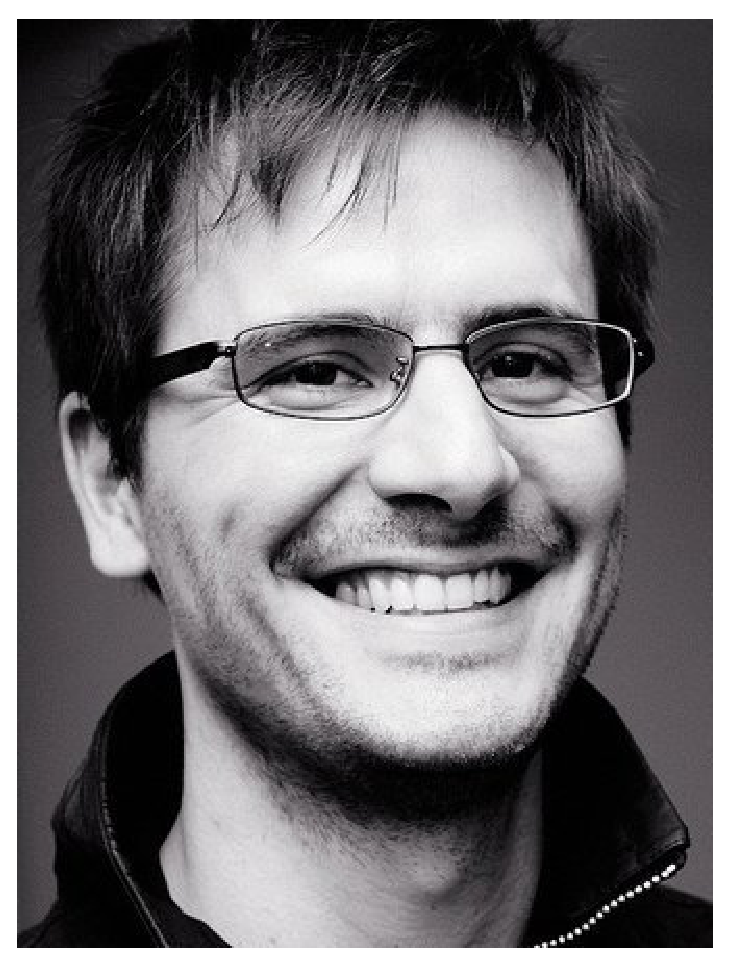
\includegraphics[width=1in,height=1.25in,clip,keepaspectratio]{figs/andresProfilePic.eps}}]{Andres Mora}
Andres Mora was born in San Jose, Costa Rica. He received his B.S. in Electronics Engineer from the Universidad Interamericana de Costa Rica and his M.Sc. and Ph.D in Aerospace Engineering (Space Robotics) in 2006 and 2009 respectively at the Space Robotics Laboratory, Tohoku University, Japan. His research interests span path planning, teleoperation and control of mobile robots in the fields of human-robot interaction, search-and-rescue and planetary exploration.
\end{IEEEbiography}

% if you will not have a photo at all:
\begin{IEEEbiographynophoto}{Colin Ho}
Biography text here.
\end{IEEEbiographynophoto}

% insert where needed to balance the two columns on the last page with
% biographies
%\newpage

\begin{IEEEbiographynophoto}{Srikanth Saripalli}
Biography text here.
\end{IEEEbiographynophoto}

% You can push biographies down or up by placing
% a \vfill before or after them. The appropriate
% use of \vfill depends on what kind of text is
% on the last page and whether or not the columns
% are being equalized.

%\vfill

% Can be used to pull up biographies so that the bottom of the last one
% is flush with the other column.
%\enlargethispage{-5in}



% that's all folks
\end{document}


